\documentclass[12pt,a4paper]{report}
\usepackage[pdftex]{graphicx} %for embedding images
\usepackage{url} %for proper url entries
\usepackage[bookmarks, colorlinks=false, pdfborder={0 0 0}, pdftitle={<pdf title here>}, pdfauthor={<author's name here>}, pdfsubject={<subject here>}, pdfkeywords={<keywords here>}]{hyperref} 
\usepackage{ctable} % for \specialrule command

\usepackage{amsmath,amsthm,amssymb,amsfonts}
\usepackage{lipsum}


\usepackage[paperheight=11.69in,paperwidth=8.27in,includefoot,top=1.18in, bottom=1.18in, left=1.58in, right=0.98in]{geometry}


\usepackage{subcaption} % two figures in one place

\usepackage{multirow}%test cases
\usepackage{float}
\usepackage{amssymb}
\newcommand{\checkbox}{$\square$}
\newcommand\fillin[1][3cm]{\makebox[#1]{\dotfill}}
%for refferennce numbering
\usepackage[nottoc,notlot,notlof]{tocbibind}
%for cant show section number
\usepackage[figurename=Fig-, tablename=Tab-, labelsep=none, labelformat={default}]{caption}%for caption number delete
%\captionsetup[table]{name=Tab}
\usepackage{CJKutf8}
\newcommand{\zh}[1]{\begin{CJK}{UTF8}{gbsn}#1\end{CJK}}
%for dot line
\usepackage{tocloft}
%\renewcommand{\cftpartleader}{\cftdotfill{\cftdotsep}} % for parts
\renewcommand{\cftsecleader}{\cftdotfill{\cftdotsep}}

%section font


%figure numbering depend on section number
\usepackage{chngcntr}
\counterwithin{figure}{section}
\counterwithin{table}{section}
%left allignment
\usepackage{ragged2e}

%font size
\usepackage[T1]{fontenc}
\usepackage[utf8]{inputenc}
\pdfmapline{= rjvnr8t Verdana " winfontsT1Encoding ReEncodeFont " <[winfonts256.enc <verdana.ttf}
\usepackage{newtxtext,newtxmath}

\usepackage{verbatim}

%tab
\newcommand\tab[1][0cm]{\hspace*{#1}}
% Code segment
\usepackage{listings}
\usepackage{color}

%Header footer
\usepackage{geometry,fancyhdr}
\pagestyle{fancy}

\fancyhf{}% Clear header/footer



%\chead{%
%  \center Bangladesh Army University of Science and Technology Graduation Design(Thesis)
%}
\cfoot{\thepage}
%\cfoot{\vspace*{-1.5\baselineskip}\thepage}
\renewcommand{\headrulewidth}{0pt}% Default \headrulewidth is 0.4pt
\renewcommand{\footrulewidth}{0pt}
%\headheight 30pt
%\footskip 70pt

\definecolor{dkgreen}{rgb}{0,0.6,0}
\definecolor{gray}{rgb}{0.5,0.5,0.5}
\definecolor{mauve}{rgb}{0.58,0,0.82}

\usepackage{array}

\newcolumntype{M}[1]{>{\centering\arraybackslash}m{#1}}
\newcolumntype{N}{@{}m{0pt}@{}}

%Title Chapter
%\usepackage{blindtext}
%\usepackage{sectsty}
%\sectionfont{\centering}

\AtBeginDocument{
  \addtocontents{toc}{\fontsize{12}{16}\fontfamily{ptm}\selectfont}
  \addtocontents{lof}{\fontsize{12}{16}\fontfamily{ptm}\selectfont}
  \addtocontents{lot}{\fontsize{12}{16}\fontfamily{ptm}\selectfont}
}

\usepackage{titlesec}
\titleformat{\chapter}[display]
    {\filcenter\normalfont\Large\bfseries}
    {\MakeUppercase{\chaptertitlename}\ \thechapter}
    {20pt}
    {}
\titlespacing*{\chapter}{0pt}{0.5in}{20pt}
\titleformat*{\section}{\bfseries\fontsize{18}{20}\fontfamily{ptm}\selectfont}
\titleformat*{\subsection}{\bfseries\fontsize{16}{20}\fontfamily{ptm}\selectfont}
\titleformat*{\subsubsection}{\bfseries\fontsize{14}{20}\fontfamily{ptm}\selectfont}
%\renewcommand\cftsecfont{\fontsize{32}{10}\fontfamily{ptm}\selectfont }


%\makeatletter
%\renewcommand*{\@seccntformat}[1]{\csname the#1\endcsname\hspace{.5em}}
%\makeatother
%space reduce between number and section in toc
\makeatletter

\renewcommand*\l@chapter{\@dottedtocline{1}{0.2em}{0.8em}}
\renewcommand*\l@section{\@dottedtocline{1}{0.9em}{1.5em}}
\renewcommand*\l@subsection{\@dottedtocline{2}{1.7em}{2.3em}}
\renewcommand*\l@subsubsection{\@dottedtocline{3}{2.5em}{2.2em}}
\renewcommand*\l@figure{\@dottedtocline{1}{1em}{2em}}
\renewcommand*\l@table{\@dottedtocline{1}{1em}{2em}}
\renewcommand*{\@dotsep}{1}
\let\ps@plain\ps@fancy
\renewcommand*{\@seccntformat}[1]{\csname the#1\endcsname\hspace{.2em}}% for reducing space in section of section title and number
\def\fnum@figure{\figurename\thefigure}
\def\fnum@table{\tablename\thetable}
\makeatother


%Size of header of of toc tof lof
\usepackage{tocloft}
\renewcommand{\cfttoctitlefont}{\hfill\fontsize{20}{16}\fontfamily{ptm}\selectfont\bfseries}
\renewcommand{\cftaftertoctitle}{\hfill}
\renewcommand{\cftlottitlefont}{\hfill\fontsize{20}{16}\fontfamily{ptm}\selectfont\bfseries}
\renewcommand{\cftafterlottitle}{\hfill}
\renewcommand{\cftloftitlefont}{\hfill\fontsize{20}{16}\fontfamily{ptm}\selectfont\bfseries}
\renewcommand{\cftafterloftitle}{\hfill}

%\renewcommand{\thetable}{\hspace{.1em}} %table number out

% reduce space betn two vertical line
\usepackage{setspace}
%\onehalfspacing
\renewcommand{\baselinestretch}{1}
\setlength{\parskip}{0.25cm}
\setlength{\parindent}{4em}

\lstset{frame=tb,
  language=Java,
  aboveskip=3mm,
  belowskip=3mm,
  showstringspaces=false,
  columns=flexible,
  basicstyle={\small\ttfamily},
  numbers=none,
  numberstyle=\tiny\color{gray},
  keywordstyle=\color{blue},
  commentstyle=\color{dkgreen},
  stringstyle=\color{mauve},
  breaklines=true,
  breakatwhitespace=true,
  tabsize=3
}
\usepackage{times} % For times new roman


\renewcommand{\bibname}{References}

%\renewcommand{\thesection}{\thechapter.\arabic{section}} %for chapter show

\begin{document}
	%\captionsetup[figure]{labelformat={default},labelsep=none,name={Fig}}
	
	
	%\renewcommand\bibname{References} 		%Renames "Bibliography" to 				"References"
	%\begin{titlepage}
\begin{center}
	\centering
	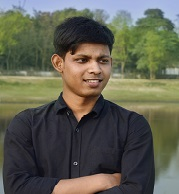
\includegraphics[width=0.15\textwidth]{/home/basedul/Documents/Report-writing-using-latex/ResturentManagementSystemReport/BasedulAppIcon.png}\par\vspace{1cm}
	{\scshape\LARGE Columbidae University \par}
	\vspace{1cm}
	{\scshape\Large Final year project\par}
	\vspace{1.5cm}
	{\huge\bfseries Pigeons love doves\par}
	\vspace{2cm}
	{\Large\itshape John Birdwatch\par}
	\vfill
	supervised by\par
	Dr.~Mark \textsc{Brown}

	\vfill

% Bottom of the page
	{\large \today\par}
\end{center}
\end{titlepage}
	%height=4in
	
	
	
%	\begin{titlepage}
%	\begin{center}
%	\centering
%	\noindent\begin{minipage}{0.25\textwidth}% adapt widths of minipages to your needs
%
\includegraphics[width=\linewidth]{/home/basedul/Documents/Report-writing-using-latex/HouseRentalManagementSystem/Uni-logo/baust-update-logo.png}
%\end{minipage}
%\hfill
%\begin{minipage}{0.7\textwidth}
%%\raggedleft
%{\fontsize{24}{5}\fontfamily{ptm}\selectfont \textbf{GRADUATION THESIS}
%}
%
%\end{minipage}
%	
%\par\vspace{0cm}
%	{\fontsize{25}{12}\fontfamily{ptm}\selectfont \begin{center}
%	\textbf{House Rental Management System}
%	\end{center}}
%%	{\fontsize{20}{10}\fontfamily{ptm}\selectfont \begin{center}
%%	\zh{亚洲餐厅管理应用}
%%	\end{center}}
%	\vspace{.5cm}
%	
%	\begin{table}[ht]
%	\center
%	\begin{tabular}{M{3.5cm}M{8cm}N}
%	
%	{\fontsize{16}{10}\fontfamily{ptm}\selectfont \begin{flushleft}
%	Department
%	\end{flushleft}} & {\fontsize{16}{10}\fontfamily{ptm}\selectfont \begin{flushleft}
%	Computer Science and Technology
%	\end{flushleft}}&\\[0.1pt]
%	
%	{\fontsize{16}{10}\fontfamily{ptm}\selectfont \begin{flushleft}
%	Degrees
%	\end{flushleft}} & {\fontsize{16}{10}\fontfamily{ptm}\selectfont \begin{flushleft}
%	Bachelor of Science
%	\end{flushleft}}&\\[0.1pt]
%	
%%	{\fontsize{16}{10}\fontfamily{ptm}\selectfont \begin{flushleft}
%%	Student No.
%%	\end{flushleft}} & {\fontsize{16}{10}\fontfamily{ptm}\selectfont \begin{flushleft}
%%	14031274
%%	\end{flushleft}}&\\[0.1pt]
%	
%	\fontsize{16}{10}\fontfamily{ptm}\selectfont{\begin{flushleft}
%	Name
%	\end{flushleft}} & \fontsize{16}{10}\fontfamily{ptm}\selectfont{\begin{flushleft}
%	Md. Basedul isam, Chow. Wasif hossain
%	\end{flushleft}}&\\[0.1pt]
%	
%	\fontsize{16}{10}\fontfamily{ptm}\selectfont{\begin{flushleft}
%	Supervisor
%	\end{flushleft}} & \fontsize{16}{10}\fontfamily{ptm}\selectfont{\begin{flushleft}
%	Al-Hasan
%	\end{flushleft}}&\\[0.1pt]
%	
%	\end{tabular}
%	\end{table}	
%	
%	
%	\vspace{1cm}
%	{\fontsize{15}{10}\fontfamily{ptm}\selectfont \MakeUppercase{Bangladesh Army University of Science and Technology} \par}
%	\vspace{0.5cm}
%	\begin{comment}\vspace{1cm}
%	{\scshape\Large Final year project\par}
%	\vspace{1.5cm}\end{comment}
%	
%	%{\Large\itshape Hossain Syed Abir\par}
%	\begin{comment}\vfill
%	Supervised by\par
%	\textsc{Liang Zhao}
%
%	\vfill
%	\end{comment}
%
%% Bottom of the page
%	{\fontsize{16}{1}\fontfamily{ptm}\selectfont July 2019\par}
%\end{center}
%\end{titlepage}

% For al-hasan sir format-title:
\begin{titlepage}
	\center
	{\fontsize{16}{10}\fontfamily{ptm}\selectfont \textbf{House Rental Management System}}\\
	\vspace{.5in}
	{\fontsize{12}{10}\fontfamily{ptm}\selectfont by}\\
	\vspace{.5in}
	{\fontsize{12}{16}\fontfamily{ptm}\selectfont 
	Md. Basedul islam\\ID: 150101093\\Chowdhury Wasif Hussain\\ID: 150101052}\\
	\vspace{1.2in}
	{\fontsize{12}{16}\fontfamily{ptm}\selectfont 
	BACHELOR OF SCIENCE IN COMPUTER SCIENCE AND ENGINEERING}\\
	\vspace{1in}
	\begin{minipage}{0.25\textwidth}% adapt widths of minipages to your needs

\includegraphics[width=\linewidth]{/home/basedul/Documents/Report-writing-using-latex/HouseRentalManagementSystem/Uni-logo/baust-update-logo.png}
\end{minipage}\\
\vspace{1in}
	{\fontsize{12}{10}\fontfamily{ptm}\selectfont Department of Computer Science and Engineering}\\
	\vspace{.5em}
	{\fontsize{12}{10}\fontfamily{ptm}\selectfont Faculty of Computer and Electrical Engineering}\\
	\vspace{.5em}
	{\fontsize{12}{10}\fontfamily{ptm}\selectfont BANGLADESH ARMY UNIVERSITY OF SCIENCE AND TECHNOLOGY}\\
	\vspace{.5em}
	{\fontsize{12}{10}\fontfamily{ptm}\selectfont June 2019}
	
\end{titlepage}


%\begin{titlepage}
%	\center
%	{\fontsize{14}{10}\fontfamily{ptm}\selectfont\textbf{House Rental Management System}}\\
%	\vspace{.8in}
%	{\fontsize{12}{10}\fontfamily{ptm}\selectfont This thesis is submitted in partial fulfillment of the requirement for the degree of Bachelor of Science in Computer Science \& Engineering.}\\
%	\vspace{.8in}
%	{\fontsize{12}{10}\fontfamily{ptm}\selectfont By}\\
%	{\fontsize{14}{10}\fontfamily{ptm}\selectfont Md. Basedul Islam}\\
%	{\fontsize{12}{10}\fontfamily{ptm}\selectfont ID: 150101093}\\{\fontsize{14}{10}\fontfamily{ptm}\selectfont Chowdhury Wasif Hussain}\\
%	{\fontsize{12}{10}\fontfamily{ptm}\selectfont ID: 150101052}\\
%	\vspace{.8in}
%	{\fontsize{12}{16}\fontfamily{ptm}\selectfont Supervised by\\Mr. Md. Al-Hasan\\Lecturer\\Department of Computer Science \& Engineering(CSE)\\Bangladesh Army University of Science \& Technology}\\
%	\vspace{1.2in}
%	{\fontsize{12}{10}\fontfamily{ptm}\selectfont \textbf{July, 2019}}\\
%	\vspace{.5em}
%	{\fontsize{16}{10}\fontfamily{ptm}\selectfont \textbf{Department of Computer Science \& Engineering}}\\
%	\vspace{.5em}
%	{\fontsize{14}{10}\fontfamily{ptm}\selectfont \textbf{Bangladesh Army University of Science and Technology}}\\
%	\vspace{.5em}
%	{\fontsize{12}{10}\fontfamily{ptm}\selectfont \textbf{Saidpur(Cantonment), Nilphamari}}
%\end{titlepage}

\begin{titlepage}
	\pagenumbering{Roman}
%	\setcounter{page}{1}
	\thispagestyle{fancy}
	\RaggedRight\justify{ The thesis titled \textbf{“House Rental Management System”} submitted by Roll No.150101052, 150101093, Session 2015-2019 has been accepted as satisfactory in fulfillment of the requirement for the degree of Bachelor of Science in Computer Science \& Engineering (CSE) as B.Sc. Engineering to be awarded by the Bangladesh Army University of Science \& Technology.}
	{\center
	\vspace{.3in}
	{\fontsize{16}{10}\fontfamily{ptm}\selectfont\textbf{Board of Examiners}}\\
	\vspace{.5in}}
	\RaggedRight ---------------------------------------\\
	Prof. Dr. Md. Mamunur Rashid\hspace{17em} Chairman\\
	Professor\\
	Head, Dept. of CSE, BAUST.
	\vspace{.5in}\\
	\RaggedRight ---------------------------------------\\
	Mr. Md. Al-Hasan\hspace{22em} Supervisor\\
	Lecturer\\
	Dept. of CSE, BAUST.
	\vspace{.5in}\\
	\RaggedRight ---------------------------------------\\
	Dr. S.M Sadakatul Bari\hspace{21em} Member\\
	Assistant Professor\\
	Dept. of CSE, BAUST.
	\vspace{.5in}\\
	\RaggedRight ---------------------------------------\\
	\RaggedRight Mr. Md. Moazzem Hossain\hspace{19em} Member\\
	Lecturer\\
	Dept. of CSE, BAUST.
	\vspace{.5in}\\
	\RaggedRight ---------------------------------------\\
	Ms. Sumya Akter\hspace{23em} Member\\
	Lecturer\\
	Dept. of CSE, BAUST.
	\vspace{.5in}\\\newpage
	\RaggedRight ---------------------------------------\\
	Ms. Fatima-Tuz-Zohra\hspace{20.8em} Member\\
	Lecturer\\
	Dept. of CSE, BAUST.
	\vspace{.5in}\\
	\RaggedRight ---------------------------------------\\
	Ms. Tarana Ara\hspace{23.5em} Member\\
	Lecturer\\
	Dept. of CSE, BAUST.
	\vspace{.5in}\\
	\RaggedRight ---------------------------------------\\
	Mr. Hasan Muhammad kafi\hspace{18.8em} Member\\
	Lecturer\\
	Dept. of CSE, BAUST.
	\vspace{.5in}\\
	\RaggedRight ---------------------------------------\\
	Dr. Mohammad Sowket Ali\hspace{18.5em} Member\\
	Assistant Professor\hspace{21.8em} (External)\\
	Dept. of CSE, BAUST.
	
	\newpage
	\clearpage\mbox{}\clearpage
	\begin{center}
	\MakeUppercase{\textbf{Candidate's Declaration}}
	\end{center}
	{\RaggedRight\justify It is hereby declared that this thesis/project or any part of it has not been submitted elsewhere for the award of any degree or diploma.}\\
	
	\vspace{5em}
	\hspace{20.5em}Signature of the Candidates\\
	\vspace{2em}
	\hspace{18em}------------------------------------------------\\
	\hspace{19.5em}Md. Basedul Islam(150101093)\\
	\vspace{2em}
	\hspace{18em}------------------------------------------------\\
	\hspace{18em}Chowdhury Wasif Hussain(150101052)	
	
	
	\newpage
	\begin{center}
	\textbf{DEDICATION}
	\end{center}
	\vspace{.2em}
	\begin{center}
	I dedicate this thesis/project to our parents \& teachers.
	\end{center}
\end{titlepage}

	\thispagestyle{fancy}
	\setcounter{page}{6}
	\tableofcontents\thispagestyle{fancy}\newpage
	\listoffigures\thispagestyle{fancy}\newpage
	\listoftables\thispagestyle{fancy}\newpage
	%\pagenumbering{arabic} %reset numbering to normal for the main content
	
	\begin{titlepage}
	\vspace*{.05cm}	
		%\pagenumbering{roman} %numbering before main content starts
		\thispagestyle{fancy}
		\pagenumbering{Roman}
		\setcounter{page}{10}
		\centering 
		{\fontsize{20}{10}\fontfamily{ptm}\selectfont \textbf{Acknowledgment}}\\
		\vspace{0.6cm}
		\justify Foremost, we would like to express my sincere gratitude to the almighty Allah for His blessings and protection throughout our undergraduate studies.\\ 
our sincere thanks to our supervisor,  \textbf{Mr. Md. Al-Hasan} of the department of Computer Science and Engineering at Bangladesh Army University of Science and Technology for the continuous support of our Bachelor's study, patience, motivation, enthusiasm, and immense knowledge. His guidance helped us in all the time of research and writing of this thesis. We could not have imagined having a better adviser and mentor. We also thank our fellow classmates, our friends and for all the fun we have had in the last four years.
        Last but not the least; We would like to thank our parents for their prayers, support, encouragement and their admonishment. 
		
	\newpage
	
	\centering 
	
		{\fontsize{20}{10}\fontfamily{ptm}\selectfont \textbf{Abstract}}\\
		\vspace{0.6cm}
		\justify \tab  The project House Rental Management System is implemented to reduce the
manual work and enhances the accuracy of work for renting. This system has been made
in a user friendly interface. This project is also designed with full consideration to help the
users in an easy manner without any unnecessary wastage of time. It could be House, Hotel or Car. Searching a house for renting is a
tough task in Bangladesh. To make it easier we are trying to make a website where people can rent
their affordable house right sitting on their present home without roaming around for searching it.
On the other hand, if someone is going for a trip to somewhere, they can rent their hotel room just
like they did rent their house. They can also rent a car from our website.
Moving home isn’t an easy task but being prepared can help to make the process smoother,
saving you time and unnecessary stress.
This guide to renting aims to provide you with the advice you’ll need to get the most out of renting
as well as reassurance with answers to common problems and questions. Bangladeshi rental market
has grown significantly over the past few years.\\

\RaggedRight{\bfseries Key Words: } House Rental Management System, PHP, HTML, CSS, JavaScript, Wamp server, MySQL, Database.

%\newpage
%\centering 
%	{\fontsize{16}{10}\fontfamily{ptm}\selectfont \textbf{Statement of Originality}}\\
%	\vspace{0.6cm}
%		\justify It is hereby declared that the contents of this project is original and any part of it has not been submitted elsewhere for the award if any degree or diploma.
%		\vspace{5in}\\
%		\textbf{Signature of the Supervisor}\hspace{2.87in}\textbf{Signature of the Candidate}\vspace{.2in}\\
%		\textbf{Date:}\hspace{4.45in}\textbf{Date:}
	\end{titlepage}
	
	
		\newpage
		\chapter{Introduction}
%		\section{Introduction}
		\pagenumbering{arabic}
		%{\bfseries \Large INTODUCTION}\\
		\tab{Searching for a suitable house for rent has become a painful job especially in crowded cities like Dhaka.
	Both the landlords and rent seekers faces trouble to get the right thing. Now a days the Bangladesh
	government has also keep track of every people in every flat/house. But this is also becoming a tough task
	to keep the right record each time as they relocating quickly to a new flat/house for their job.
	We worked in such home rental system to build a more dynamic system than the existing ones. Our
	goal of this thesis is to make the system as user-friendly as possible. For this purpose, we have shrunk
	the whole in via an icon in the mobile phones as well so that the users can search for vacant houses
	and transport at any time. To minimize any kind of communication gap, we introduce a chatting system
	between agents and admin. Users always want to get a result in the shortest span of time. In many
	cases, may be users get the reply lately due to internal long manual processes. To solve that, we
	introduce a dynamic mail system to notify the user's search result in the least possible time. Therefore,
	the home rental system holds features like rental search, dynamic mail system, tenants can search for
	vacant houses randomly according to their wishes based on unique area or city, they can track for
	vehicles from their given location as well. Additionally, they can add their wish list if their desired
	home is not available. There will be a chat system in which admin and agent can chat directly. All the
	values which are used for processing result are dynamic in our home rental system. In our system, there
	is an option whether u want family house or bachelor. However, recently it has become a trivial issue
	for the bachelors because none of the house owners are ready to rent their houses to them. Therefore,
	we create such a safe and user-friendly platform for the bachelors so that they can rent house efficiently
	and, in a hassle, free procedure. Roam around to rent a house has always been a hassle for people. Especially, on recent times, people have so many priorities based on which they have to rent their house. Some people want their house to be in the commercial space, or some want in a chaos free space. Some people prefer to choose the area of their house relating the religion they belong. Again there are a lot of people who love pets; therefore they want a house which has pet allowance. Basically, in this era of modernism people want to rent their house like online shopping. To rent a house in physical world has become less popular now a days [1]. No one wants to roam around here and there to search for a house. People would prefer a virtual system to rent a house. To decode this situation and to represent a hassle free environment to the people, a dynamic system can be implemented. That system would give the tenants the best service for renting houses without any kind of hassle. Government can make one unique system where people can rent house based on their priority instead of having so many rental systems. In that system, all the vacant houses of any district of Bangladesh will be listed there. One system will hold every details of every vacant house from any district, any are. To, make the system more liable, there should be a system by which tenants can verify the owner or agent. Also, to analysis the place they will rent for house they need to know the location of that. Hence, every information details which have minimum priority to rent a house will hold by the system. There a one special feature for the bachelors so that they can rent houses efficiently as now a days house owners do not want to rent their houses to the bachelors for safety issue. People can rent hotels and cars too.}
		\section{The problem}
		\tab{Roam around to rent a house has always been a hassle for people. Especially, on recent times, people
	have so many priorities based on which they have to rent their house. Some people want their house to
	be in the commercial space, or some want in a chaos free space. Some people prefer to choose the area
	of their house relating the religion they belong. Again, there are a lot of people who love pets; therefore,
	they want a house which has pet allowance. Basically, in this era of modernism people want to rent
	their house like online shopping. To rent a house in physical world has become less popular now a
	days \cite{Ref:1} one wants to roam around here and there to search for a house. People would prefer a
	virtual system to rent a house.\\
	To decode this situation and to represent a hassle-free environment to the people, a dynamic system
	can be implemented. That system would give the tenants the best service for renting houses without
	any kind of hassle. Government can make one unique system where people can rent house based on
	their priority instead of having so many rental systems. In that system, all the vacant houses of any
	district of Bangladesh will be listed there. One system will hold every details of every vacant house
	from any district, any are. To, make the system more liable, there should be a system by which tenants
	can verify the owner or agent. Also, to analysis the place they will rent for house they need to know
	the location of that. Hence, every information details which have minimum priority to rent a house will
	hold by the system. There a one special feature for the bachelors so that they can rent houses efficiently
	as now a day house owner does not want to rent their houses to the bachelors for safety issue.}
		\section{Project objectives}
	\tab{According to the universal declaration of human rights by which we get to know that is belong to a
	human the right to have a proper standard of living. (United Nations, The Human Rights-article 25,
	1948).\cite{Ref:1} A standard living place is every citizen’s basic right. Choosing that place is also their right.
	As technology is growing so fast every single day, it is necessary to make the system the most dynamic
	approach. By the need of this, a dynamic home rental system is needed where every citizen can choose
	their house according to their choice and also it has to be most dynamic as people will access this
	system at anytime from anywhere.\\
	Targeting these issues in manual house rental management system, we are proposing an automated
	rental management system where the bellow three stakeholders will be benefited greatly-
	\begin{itemize}
		\item Landlords
		\item Rent Seeker
		\item The government
	\end{itemize}
	Our project is about Renting House. Searching a house for renting is a tough task in Bangladesh.
	To make it easier we are trying to make a website where people can rent their affordable house
	right sitting on their present home without rooming around for searching it.\\
	Moving home isn’t an easy task but being prepared can help to make the process smoother,
	saving you time and unnecessary stress.\\
	This guide to renting aims to provide you with the advice you’ll need to get the most out of renting as well
	as reassurance with answers to common problems and questions. Bangladeshi rental market has grown
	significantly over the past few years.
	Though once reserved only for students or those unable to purchase, renting has become an increasingly
	attractive alternative to buying by providing a number of unique benefits such as:
	\begin{itemize}
		\item \textbf{Flexibility}-when you rent you agree to stay in a property for a fixed length, usually 12 months,
	meaning that you are free to move elsewhere if you want.
		\item \textbf{Cost}-because you do not own the property you are not liable for property maintenance costs or
	replacing expensive items such as boilers.
	\end{itemize}
	Most popular in larger towns and cities, renting in the Bangladesh is often the first step for most after
	moving out of their family home.
	Though currently not as heavily regulated as the resale and buying market, many new rules have come into
	effect over the last couple of years providing greater protection for tenants.
	While the majority of tenants will never experience a problem with their tenancy or landlord, it’s
	important to understand what’s usual (and what’s not) and what’s expected from both parties.}
	
		\section{Project requirements analysis}
		\tab{Project requirements analysis are important stage in the system development. It
	determines the functions of the whole application integrity and stability. Software requirements
	analysis is an ongoing process of understanding and progressive refinement. Through
	requirements analysis, design functions of the management system as below-}
				\begin{itemize}
					\item[a.]\textbf{User management:} User can sign up (client), sign in and sign out the application.
					\item[b.]\textbf{Adding a house:} admin can add new house information for showing to clients.
					\item[c.]\textbf{House's information browsing:} The house's are grouped by categories. Clients may
	browse the detailed information of a house.
					\item[d.]\textbf{house query:} admin can query house's according to price, name.
					\item[e.]\textbf{house comments:} clients can write comments on the house.
				\end{itemize}
			\subsection{Requirements analysis}
			\tab{The in-front management system is the user visits home list and
	sign up user as client. Only the admin can manage his/her searching potion about the
	specific home, comment and price. So in this part, specific functions are described as
	below:}	\begin{itemize}
					\item {\bfseries Sign in and Sign out:} User can sign in into system and also sign out from the system.
					\item {\bfseries Register:} If user have no account, user have to must create an account.
					\item {\bfseries Modify personal information:} User can also modify his personal information.
					\item {\bfseries Browse detailed information of a home:} User can browse details of home.
					\item {\bfseries Comments:} User can post a comment for each home.
				\end{itemize}
			\section{Project deliverable's}
	\tab{Deliverables\cite{Ref:2} are usually classified as internal deliverables and external deliverables.}\\
	Internal deliverables :  Internal deliverables are usually deliverables that make a project run, but they are not a part of the product that the end users would like to see. They are deliverables which the project generates internally. Project Management, Configuration Management, Training and Testing are some examples of internal deliverables.\\
	External Deliverables : External deliverables are usually those that the project delivers to the users or the client. An external deliverable could be an IT system and subsystems that make it up or the resulting organizational transition and benefits from a project to reduce the turnaround time of a process.\\
	{The main deliverable of this project is to build a simple and easy use of House Rental Management System following the specific software requirements as well as the programming languages.}\\
		\begin{itemize}
			\item Functioning software application.
			\item List of (non) functional requirement.
			\item Schematic models (analysis+design).
			\item Evaluation findings.
			\item Dissertation report.
		\end{itemize}
\newpage
\chapter{Background Study}	
Roam around to rent a house has always been a hassle for people. Especially, on recent times,
people have so many priorities based on which they have to rent their house.
The main goal of our project is to make life easier for renters and landlords. Landlords can
upload their rent-able houses sample on our website and rent price and renters will rent if its
affordable for them. Our other goal is to help our law enforcement organization by keeping the
necessary information of a renter for initial verification. It will help to reduce crime in our
country.
There are some websites like us which are currently working to solve the problem. Here we will
discuss about it and we will also show the difference between there sites and ours.
\section{Airbnb}
Airbnb is one of the leading online house rental sites which has grown into the largest brand in
just a span of a decade. The company’s state-of-the-art platform aids all its stakeholders
including employees, guests, hosts, and the communities.  By uniquely leveraging innovative
technologies, Airbnb aids millions of people across the world to rent out and monetize their extra
spaces. Airbnb currently provides access to more than 5 million accommodations in over 81,000
cities across 191 countries. Founded in 2008, Airbnb was formerly known as Airbed and
Breakfast and is currently based in San Francisco, California.
\section{Upad}
Founded in 2008 by James Davis, Upad has become the UK’s largest online house rental agency,
disrupting the traditional letting agent model. Upad is one of the perfect start-up examples where
technology innovation is leveraged to boost the property industry, also termed as ‘Proptech’. The
company’s services include property listing, floor planning, photography, tenant referencing,
property management, and insurance. Upad has provided its services to more than 12,500
landlords and has helped let 30,000+ properties for rent in the UK. The company allows
landlords to advertise their property on Right-move.com and Zoopl.com within 24 hours.
\section{Zumper}
Zumper creates an efficient and transparent end-to-end marketplace for making renting
apartments easy for both tenants and landlords. Their cutting-edge online house rental site
provides an easy way for people to find updated listings of apartments, which can be filtered
based on price range, pet requirements, desired amenities, location, bedroom count, and more. Zumper is supported by top investors including Goodwater Capital, The Blackstone Group,Foxhaven Asset Management, CrunchFund, xfund, Breyer Capital, Kleiner Perkins, Greylock, Partners, Andreessen Horowitz, Marcus \& Millichap, Stereo Capital, and Dawn Capital. Their
website is visited by more than 8 million people a month.
\section{Varadeal.com}
This is the only site from Bangladesh. Here anyone can upload their house and anyone can use
this site to find there preferred house to live in. But it doesn’t have any review system from the
tenants which don’t help the others to find there house. Besides anyone can upload house for rent
without any verification which creates more chances of fake accounts and hassle for tenants.
Most of this websites are from foreign countries. Very few are available from Bangladesh but
those also are not perfectly fine. Besides these websites don’t work with the government. We are
looking to improve all these problems in by creating this website.
\newpage
\chapter{System design}
%{\bfseries \Large System Design}\\
\tab{System design \cite{Ref:10} is the process of defining the elements of the system such as the
architecture, modules and components, the different interfaces of those components and
the data that goes through the system.It is meant to satisfy specific needs and requirements of a business or organization through the engineering of a coherent and well-running system.Systems design implies a systematic approach to the design of a system. It may take a bottom-up or top-down approach, but either way the process is systematic wherein it takes into account all related variables of the system that needs to be created from the architecture, to the required hardware and software, right down to the data and how it travels and transforms throughout its travel through the system. Systems design then overlaps with systems analysis, systems engineering and systems architecture.
The systems design approach first appeared right before World War II, when engineers were trying to solve complex control and communications problems. They needed to be able to standardize their work into a formal discipline with proper methods, especially for new fields like information theory, operations research and computer science in general.
}
\section{Architectural design}
\tab A system architecture \cite{Ref:11} design is the conceptual model that defines the structure, behavior, and more views of a system. An architectural description is a formal description and representation of a system, organized in a way that supports reasoning about the structures and behaviors of the system.One can think of system architecture as a set of representations of an existing (or future) system. These representations initially describe a general, high-level functional organization, and are progressively refined to more detailed and concrete descriptions.System architecture conveys the informational content of the elements consisting of a system, the relationships among those elements, and the rules governing those relationships. The architectural components and set of relationships between these components that an architecture description may consist of hardware, software, documentation, facilities, manual procedures, or roles played by organizations or people.{In this part, system block diagram details are given.Various organizations can define systems architecture in different ways, including:\begin{itemize}
	\item The fundamental organization of a system, embodied in its components, their relationships to each other and to the environment, and the principles governing its design and evolution.
	\item An allocated arrangement of physical elements which provides the design solution for a consumer product or life-cycle process intended to satisfy the requirements of the functional architecture and the requirements baseline.
	\item An architecture consists of the most important, pervasive, top-level, strategic inventions, decisions, and their associated rationales about the overall structure (i.e) essential elements and their relationships) and associated characteristics and behavior.
	\item A formal description of a system, or a detailed plan of the system at component level to guide its implementation.
	\item The composite of the design architectures for products and their life-cycle processes.
	\item The structure of components, their interrelationships, and the principles and guidelines governing their design and evolution over time.
\end{itemize}According to requirements
gather, the House Rental Management System will be designed as below:}
	\begin{figure}[H]
		\centering
		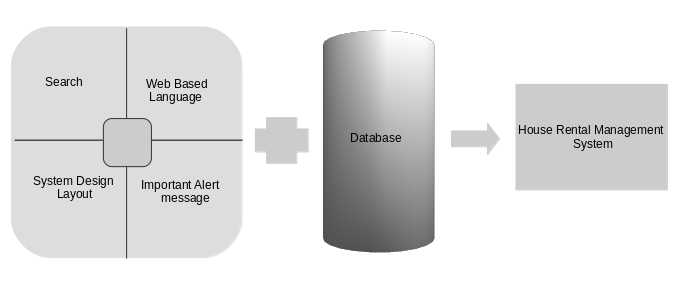
\includegraphics[height=2.5in]{/home/basedul/Documents/Report-writing-using-latex/HouseRentalManagementSystem/Architectural-design/arc-design.png}
		\caption{\hspace{0.35em}Architecture of House Rental Management System}
		\label{fig:archi} 
	\end{figure}
		
	\RaggedRight{As shown Fig-\ref{fig:archi}, the tools has been used to built the architecture of the system is html
(hypertext markup language), javascript, css (cascading style sheet), php and mysql.\\We have tried to achieve the following features in our select problem domain of designing a modern dynamic home rental application-
		\begin{itemize}
			\item Rental search
			\item Rental posting
			\item Chat server
			\item Wish list
			\item Mail alert system
			\item Google map view
			\item A responsive application of the system wev view.
		\end{itemize}
}
\section{Database diagram}
	\justify\tab Within a database diagram \cite{Ref:12}, each relationship can appear with three distinct features: endpoints, a line style, and related tables.\\
\textbf{Endpoints} The endpoints of the line indicate whether the relationship is one-to-one or one-to-many. If a relationship has a key at one endpoint and a figure-eight at the other, it is a one-to-many relationship. If a relationship has a key at each endpoint, it is a one-to-one relationship.\\
\textbf{Line Style} The line itself (not its endpoints) indicates whether the Database Management System (DBMS) enforces referential integrity for the relationship when new data is added to the foreign-key table. If the line appears solid, the DBMS enforces referential integrity for the relationship when rows are added or modified in the foreign-key table. If the line appears dotted, the DBMS does not enforce referential integrity for the relationship when rows are added or modified in the foreign-key table.\\
\textbf{Related Tables} The relationship line indicates that a foreign-key relationship exists between one table and another. For a one-to-many relationship, the foreign-key table is the table near the line's figure-eight symbol. If both endpoints of the line attach to the same table, the relationship is a reflexive relationship.

	\subsection{Entity diagram}
	\tab An Entity Relationship (ER) Diagram \cite{Ref:13} is a type of flowchart that illustrates how “entities” such as people, objects or concepts relate to each other within a system. ER Diagrams are most often used to design or debug relational databases in the fields of software engineering, business information systems, education and research. Also known as ERDs or ER Models, they use a defined set of symbols such as rectangles, diamonds, ovals and connecting lines to depict the interconnections of entities, relationships and their attributes. They mirror grammatical structure, with entities as nouns and relationships as verbs.\\
%{These diagrams below show how the attributes are defined in database table:}\\
As shown in Fig-\ref{fig:adminreg} if admin wants to check the order list from an client and add new house, admin must first signup with name, user name, email and password. After registration, he will be able to check the order list after signin, else he can not even see the order list and he will not be able to add house to the house list . 
	\begin{figure}[H]
		\centering
		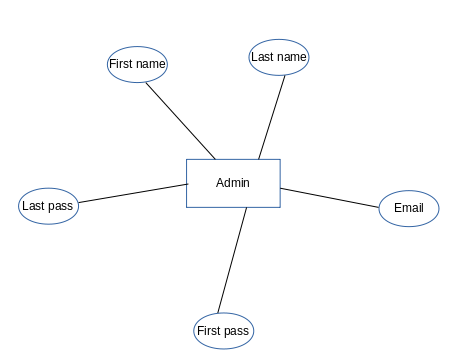
\includegraphics[height=2.5in]{/home/basedul/Documents/Report-writing-using-latex/HouseRentalManagementSystem/admin_arc_design/admin-arc.png}
		\caption{\hspace{0.35em}Admin entity diagram}
		\label{fig:adminreg} 
	\end{figure}{As shown in Fig-\ref{fig:clientreg} client can browse about house name, price and details from house list. But if client wants to place an order, client must need to sign up first with client name, username, e-mail and password and then sign in with his username and password. After logging in, he can order the house from the house category. After ordering, client can be able to sign out.}
	\begin{figure}[H]
		\centering
		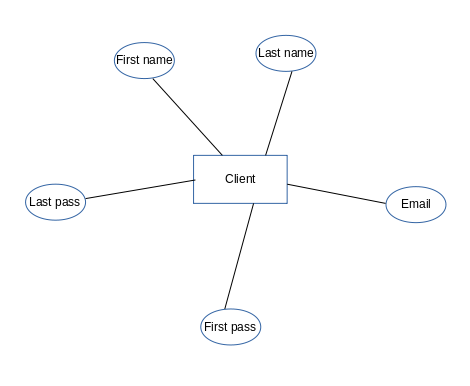
\includegraphics[height=3.5in]{/home/basedul/Documents/Report-writing-using-latex/HouseRentalManagementSystem/admin_arc_design/client-arc.png}
		\caption{\hspace{0.35em}Client entity diagram}
		\label{fig:clientreg} 
	\end{figure}
	{As shown in Fig-\ref{fig:houseadd} if admin wants to add new house items to a house list, admin must first sign up with name, user name, email and password. After registration, he will be able to check the order list after sign in, else he can not even see the order list and he will not be able to add house to the house list.}
	\begin{figure}[H]
		\centering
		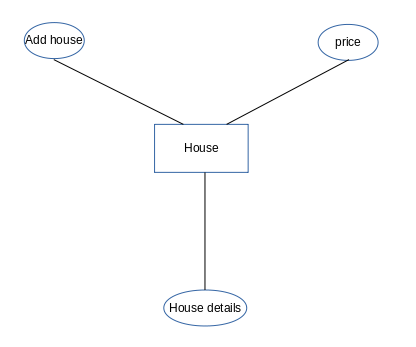
\includegraphics[height=3.5in]{/home/basedul/Documents/Report-writing-using-latex/HouseRentalManagementSystem/HouseDetails/House-details.png}
		\caption{\hspace{0.35em}House add entity diagram}
		\label{fig:houseadd} 
	\end{figure}
	
	{As shown in Fig-\ref{fig:commentsent} Client can comment on each house's and also can give reviews for a specific item of house.} 
	\begin{figure}[H]
		\centering
		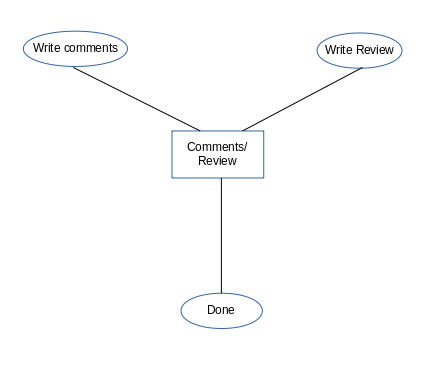
\includegraphics[height=3.5in]{/home/basedul/Documents/Report-writing-using-latex/HouseRentalManagementSystem/comments-or-reviews/comments-reveiw-arc.png}
		\caption{\hspace{0.35em}Comments/Review entity diagram}
		\label{fig:commentsent} 
	\end{figure}
	
	\subsection{E-R diagram}
		\tab An entity relationship diagram (ERD) \cite{Ref:14}, also known as an entity relationship model, is a graphical representation of an information system that depicts the relationships among people, objects, places, concepts or events within that system. An ERD is a data modeling technique that can help define business processes and be used as the foundation for a relational database.\\Entity relationship diagrams provide a visual starting point for database design that can also be used to help determine information system requirements throughout an organization. After a relational database is rolled out, an ERD can still serve as a referral point, should any debugging or business process re-engineering be needed later.\\However, while an ERD can be useful for organizing data that can be represented by a relational structure, it can't sufficiently represent semi-structured or unstructured. It's also unlikely to be helpful on its own in integrating data into a preexisting information system.\\we have described our website. Our website has two parts one for landlords and one
for Renters. To upload their house a landlord, need to sign up in our website as landlord if
someone doesn’t sign up he/she can not upload their house or hotel. Once the house is rented to
someone they can delete it from the website.
On the other hand, Rent seekers also need to have a account on our website to take rent. They can
not take any rent without singing up in our website. To match there’s preferences they can search
by their preferences like location, number of room, number of family member etc.
	
		\begin{figure}[H]
		\centering
		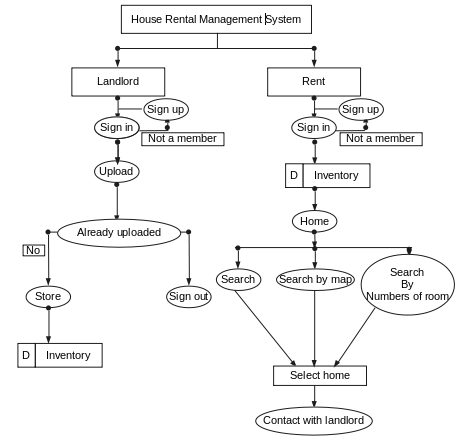
\includegraphics[height=4.5in]{/home/basedul/Documents/Report-writing-using-latex/HouseRentalManagementSystem/Entity-diagram/entity-diagram.png}
		\caption{\hspace{0.35em}ER diagram of House Rental Management System}
		\label{fig:erdig} 
	\end{figure}
	
    \subsection{Landlords}
    \tab In fig-\ref{fig:landlord-dfd} we have described our activity diagram of landlord. A landlord need to sign up an account on
our website to upload their house for rent. They also need to give a description of their house like where
its located, how many rooms available, do they allow bachelors or not etc. If they get a renter which
meets their desires they need to mark the house as unavailable for others.	
			\begin{figure}[H]
				\centering
				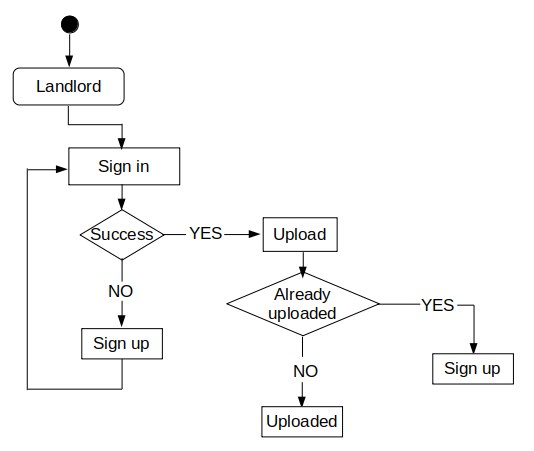
\includegraphics[height=3.5in]{/home/basedul/Documents/Report-writing-using-latex/HouseRentalManagementSystem/Report_for_House_rental_system/landlord_activity_diagram.png}
				\caption{\hspace{0.35em}Activity diagram of Landlords}
				\label{fig:landlord-dfd} 
			\end{figure}
			
	\subsection{Rent Seekers}
	\tab In fig-\ref{fig:rent-dfd} we have described the activity diagram of rent seekers. A rent seeker also should have an
account on our website in term to rent any house from our website. After signing in a rent seeker can
search randomly or they can search by their desire wishes like any specific location, by the number of
rooms, bachelor or family etc. Once they find their desired house they can chat with the landlord of that
house or they can also contact with the admin of our website.
			\begin{figure}[H]
				\centering
				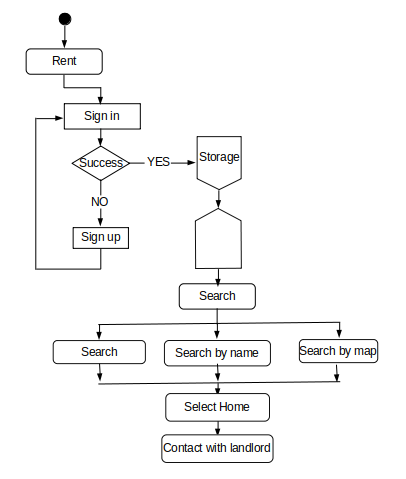
\includegraphics[height=4.5in]{/home/basedul/Documents/Report-writing-using-latex/HouseRentalManagementSystem/Report_for_House_rental_system/rent_activitydiagram.png}
				\caption{\hspace{0.35em}Activity diagram of Rent seekers}
				\label{fig:rent-dfd} 
			\end{figure}
			
			
			\subsection{Government}
	\tab In fig-\ref{fig:govt-dfd} we have described our activity diagram for our law enforcement agencies.They don't need to have a user account in our website but they need to have a specific e-mail and password given by us to get access to the website.After logging in they can only access the customer list and address.Which will help to keep crime rate under control. 
			\begin{figure}[H]
				\centering
				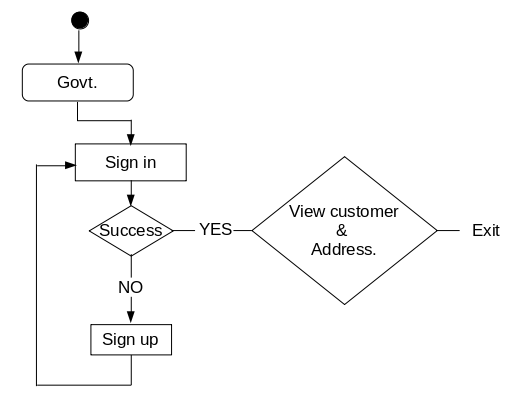
\includegraphics[height=4.5in]{/home/basedul/Documents/Report-writing-using-latex/HouseRentalManagementSystem/house-pik/govt.png}
				\caption{\hspace{0.35em}Activity diagram of Government}
				\label{fig:govt-dfd} 
			\end{figure}
			
	\section{Incremental Model}
	\tab{In fig-\ref{fig:inc-moe} Incremental model\cite{Ref:21} the whole requirement is divided into various builds. Multiple development cycles take place here, making the life cycle a “multi-waterfall” cycle.  Cycles are divided up into smaller, more easily managed modules. Incremental model is a type of software development model like V-model, Agile model etc.\\In this model, each module passes through the requirements, design, implementation and testing phases. A working version of software is produced during the first module, so you have working software early on during the software life cycle. Each subsequent release of the module adds function to the previous
		\begin{figure}[H]
					\centering
					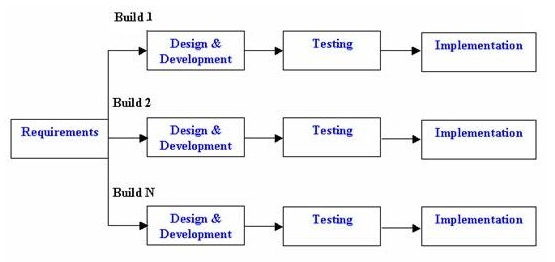
\includegraphics[height=2.5in]{/home/basedul/Documents/Report-writing-using-latex/HouseRentalManagementSystem/incrementalModel/Incremental_model.jpg}
					\caption{\hspace{0.35em}Incremental Model for House Rental Management System}
					\label{fig:inc-moe} 
				\end{figure}	
	
	}
	\section{Database schema}
%			RegistrationForAdmin(uid, uf, ul, uu, um, ufp, usp, status)\\
%			Registration(uid, uf, ul, uu, um, ufp, usp, status)\\
%			APPTIZERS(appid, appname, appprice, appdetails)\\
%			BeefLamb(blid, blname, blprice, bldetails)\\
%			Chicken(ckid, ckname, ckprice, ckdetails)\\
%			Drink(did, dname, dprice, ddetails)\\
%			NoddlesRice(nrid, nrname, nrprice, nrdetails)\\
%			Pork(poid, poname, poprice, podetails)\\
%			Salad(said, saname, saprice, sadetails)\\
%			SeaFood(sfid, sfname, sfprice, sfdetails)\\
%			Soups(soid, soname, soprice, sodetails)\\
%			VegeTofu(vtid, vtname, vtprice, vtdetails)\\
%			ClientOrderList(colid, colname, colprice, colUser)\\
%			RankList(rlid, rlname, rlscore, rlcomments)

		\tab A Database schema \cite{Ref:22} represents the logical configuration of all or part of a relational database. It can exist both as a visual representation and as a set of formulas known as integrity constraints that govern a database. These formulas are expressed in a data definition language, such as SQL. As part of a data dictionary, a database schema indicates how the entities that make up the database relate to one another, including tables, views, stored procedures, and more.Typically, a database designer creates a database schema to help programmers whose software will interact with the database. The process of creating a database schema is called data modeling When following the three-schema approach to database design, this step would follow the creation of a conceptual schema. Conceptual sachems focus on an organization’s informational needs rather than the structure of a database.

		\begin{itemize}
			\item \textbf{Registration for admin(u-id, u-f, u-l, u-u, um, ufp, usp, status):} For admin registration have a database table which have eight columns, first column is used for uniqe id, second column is used for admin's first name, third column use for admin's last name, fourth column is used for admin's user name, fifth column is used for admin's email,sixth and seventh columns is used for admin's password and last column is used for admin is active or not. 
			\item \textbf{Registration(uid, uf, ul, uu, um, ufp, usp, status):} Registration is database table which have eight columns, first column is used for unique id, second column is used for client's first name, third column use for client's last name, fourth column is used for client's user name, fifth column is used for client's email,sixth and seventh columns is used for client's password and last column is used for client is active or not. 
			\item \textbf{House upload(house name, house rent price, house details, house rent price):} For upload a house, we have a database table where given by details of house then save it.
			\item \textbf{Comments(house-id, comments):} For user comments we use a table, where store the house id and user comments.
			\item \textbf{Review(house-id, review):} For user review we use a table, where store the house id and user review.
		\end{itemize}
	
	


	\subsection{Database tables structures}
	\tab The database structure is the collection of record type and field type definitions that comprise your database. These define the type of entities or research objects you wish to capture (e.g. Person) Fields. These are the properties or attributes that describe your record types (e.g. Gender, Age, Height etc).\\
		\tab The Tab.\ref{tab:adminregitable} is used for signup a user as a admin by giving first name, last name, email and password on the application. If admin already have an account then signin in the application then manipulate the order list or add house on house list by given house name, house price and details of house.In Tab.\ref{tab:adminregitable} u-id means user uniqe id, which type is integer and default value is not null, u-f-name means user first name which type is varchar, size is 80 and default value is null, u-l-name means user last name which type is varchar, size is 80 and default value is null, u-mail means user email which type is varchar, size is 50 and default value is null, u-f-pass means first password which type is varchar, size is 20 and default value is null, u-l-pass means last password which type is varchar, size is 20 and default value is null, 
		\begin{table}[H]
		\center
	\caption{\hspace{0.4em}Admin registration}
	\label{tab:adminregitable}
	\begin{tabular}{M{0.6cm}|M{1.5cm}|M{2cm}|M{1cm}|M{1cm}|M{2.5cm}|M{3.2cm}N}
	\specialrule{.15em}{.05em}{.05em} 
	\fontsize {10}{8}\fontfamily{ptm}\selectfont {\bfseries{No}} & 
	\fontsize {10}{8}\fontfamily{ptm}\selectfont {\bfseries{Field}} & 
	\fontsize {10}{8}\fontfamily{ptm}\selectfont {\bfseries{Type}} & 
	\fontsize {10}{8}\fontfamily{ptm}\selectfont {\bfseries{Null}} & 
	\fontsize {10}{8}\fontfamily{ptm}\selectfont {\bfseries{Default}} & 
	\fontsize {10}{8}\fontfamily{ptm}\selectfont {\bfseries{Extra}} & 
	\fontsize {10}{8}\fontfamily{ptm}\selectfont {\bfseries{Description}} &\\[15pt]
	\hline
	\fontsize {10}{8}\fontfamily{ptm}\selectfont {{1}} & 
	\fontsize {10}{8}\fontfamily{ptm}\selectfont {{u-id}} & 
	\fontsize {10}{8}\fontfamily{ptm}\selectfont {{int(3)}} & 
	\fontsize {10}{8}\fontfamily{ptm}\selectfont {{No}} & 
	\fontsize {10}{8}\fontfamily{ptm}\selectfont {{None}} & 
	\fontsize {10}{8}\fontfamily{ptm}\selectfont {{Auto-increment}} & 
	\fontsize {10}{8}\fontfamily{ptm}\selectfont {{Stores the admin id}} &\\[15pt]
	\hline
	\fontsize {10}{8}\fontfamily{ptm}\selectfont {{2}} & 
	\fontsize {10}{8}\fontfamily{ptm}\selectfont {{u-f-name}} & 
	\fontsize {10}{8}\fontfamily{ptm}\selectfont {{varchar(80)}} & 
	\fontsize {10}{8}\fontfamily{ptm}\selectfont {{Yes}} & 
	\fontsize {10}{8}\fontfamily{ptm}\selectfont {{None}} & 
	\fontsize {10}{8}\fontfamily{ptm}\selectfont {{ }} & 
	\fontsize {10}{8}\fontfamily{ptm}\selectfont {{Stores the admin first name}} &\\[15pt]
	\hline
	\fontsize {10}{8}\fontfamily{ptm}\selectfont {{3}} & 
	\fontsize {10}{8}\fontfamily{ptm}\selectfont {{u-l-name}} & 
	\fontsize {10}{8}\fontfamily{ptm}\selectfont {{varchar(80)}} & 
	\fontsize {10}{8}\fontfamily{ptm}\selectfont {{Yes}} & 
	\fontsize {10}{8}\fontfamily{ptm}\selectfont {{None}} & 
	\fontsize {10}{8}\fontfamily{ptm}\selectfont {{ }} & 
	\fontsize {10}{8}\fontfamily{ptm}\selectfont {{Stores the admin last name}} &\\[15pt]
	\hline
	\fontsize {10}{8}\fontfamily{ptm}\selectfont { {5}} & 
	\fontsize {10}{8}\fontfamily{ptm}\selectfont { {u-mail}} & 
	\fontsize {10}{8}\fontfamily{ptm}\selectfont { {varchar(50)}} & 
	\fontsize {10}{8}\fontfamily{ptm}\selectfont { {Yes}} & 
	\fontsize {10}{8}\fontfamily{ptm}\selectfont { {None}} & 
	\fontsize {10}{8}\fontfamily{ptm}\selectfont { { }} & 
	\fontsize {10}{8}\fontfamily{ptm}\selectfont { {Stores the admin email}} &\\[15pt]
	\hline
	\fontsize {10}{8}\fontfamily{ptm}\selectfont { {6}} & 
	\fontsize {10}{8}\fontfamily{ptm}\selectfont { {u-f-p}} & 
	\fontsize {10}{8}\fontfamily{ptm}\selectfont { {varchar(50)}} & 
	\fontsize {10}{8}\fontfamily{ptm}\selectfont { {Yes}} & 
	\fontsize {10}{8}\fontfamily{ptm}\selectfont { {None}} & 
	\fontsize {10}{8}\fontfamily{ptm}\selectfont { { }} & 
	\fontsize {10}{8}\fontfamily{ptm}\selectfont { {Stores the admin first password}} &\\[15pt]
	\hline
	\fontsize {10}{8}\fontfamily{ptm}\selectfont { {7}} & 
	\fontsize {10}{8}\fontfamily{ptm}\selectfont { {u-l-p}} & 
	\fontsize {10}{8}\fontfamily{ptm}\selectfont { {varchar(50)}} & 
	\fontsize {10}{8}\fontfamily{ptm}\selectfont { {Yes}} & 
	\fontsize {10}{8}\fontfamily{ptm}\selectfont { {None}} & 
	\fontsize {10}{8}\fontfamily{ptm}\selectfont { { }} & 
	\fontsize {10}{8}\fontfamily{ptm}\selectfont { {Stores the admin last password}} &\\[15pt]
	\specialrule{.15em}{.05em}{.05em} 
%	\fontsize {10}{8}\fontfamily{ptm}\selectfont {u-id} & \fontsize {10}{8}\fontfamily{ptm}\selectfont {tinyint(3)} & \fontsize {10}{8}\fontfamily{ptm}\selectfont {NO} &\\[10pt]
%	\hline
%	\fontsize {10}{8}\fontfamily{ptm}\selectfont {u-f-name} & \fontsize {10}{8}\fontfamily{ptm}\selectfont {varchar(80)} & \fontsize {10}{8}\fontfamily{ptm}\selectfont {YES} &\\[10pt]
%	\hline
%	\fontsize {10}{8}\fontfamily{ptm}\selectfont {u-l-name} & \fontsize {10}{8}\fontfamily{ptm}\selectfont {varchar(80)} & \fontsize {10}{8}\fontfamily{ptm}\selectfont {YES} &\\[10pt]
%	\hline
%	\fontsize {10}{8}\fontfamily{ptm}\selectfont {u-u-name} & \fontsize {10}{8}\fontfamily{ptm}\selectfont {varchar(80)} & \fontsize {10}{8}\fontfamily{ptm}\selectfont {YES} &\\[10pt]
%	\hline
%	\fontsize {10}{8}\fontfamily{ptm}\selectfont {U-mail} & \fontsize {10}{8}\fontfamily{ptm}\selectfont {varchar(50)} & \fontsize {10}{8}\fontfamily{ptm}\selectfont {YES} &\\[10pt]
%	\hline
%	\fontsize {10}{8}\fontfamily{ptm}\selectfont {u-f-pass} & \fontsize {10}{8}\fontfamily{ptm}\selectfont {varchar(20)} & \fontsize {10}{8}\fontfamily{ptm}\selectfont {YES} &\\[10pt]
%	\hline
%	\fontsize {10}{8}\fontfamily{ptm}\selectfont {u-l-pass} & \fontsize {10}{8}\fontfamily{ptm}\selectfont {varchar(20)} & \fontsize {10}{8}\fontfamily{ptm}\selectfont {YES} &\\[10pt]
%	\hline
	\end{tabular}
	\end{table}The Tab.\ref{tab:clientregitable} is used for signup a user as a client by giving first name, last name, email and password on the application. If client already have an account then signin in the application then select the house from house list and befor confirm order must signup by given personal information after signup client signin in the system by given client email and password.In table \ref{tab:clientregitable} u-id means user unique id, which type is integer and default value is not null, u-f-name means user first name which type is varchar, size is 80 and default value is null, u-l-name means user last name which type is varchar, size is 80 and default value is null, u-mail means user email which type is varchar, size is 50 and default value is null, u-f-pass means first password which type is varchar, size is 20 and default value is null, u-l-pass means last password which type is varchar, size is 20 and default value is null,
	\begin{table}[H]
		\center
	\caption{\hspace{0.4em}Registration for client}
	\label{tab:clientregitable}
	
	\begin{tabular}{M{0.6cm}|M{1.5cm}|M{2cm}|M{1cm}|M{1cm}|M{2.5cm}|M{3.3cm}N}
	\specialrule{.15em}{.05em}{.05em}
	\fontsize {10}{8}\fontfamily{ptm}\selectfont {\bfseries {No}} & 
	\fontsize {10}{8}\fontfamily{ptm}\selectfont {\bfseries{Field}} & 
	\fontsize {10}{8}\fontfamily{ptm}\selectfont {\bfseries{Type}} & 
	\fontsize {10}{8}\fontfamily{ptm}\selectfont {\bfseries{Null}} & 
	\fontsize {10}{8}\fontfamily{ptm}\selectfont {\bfseries{Default}} & 
	\fontsize {10}{8}\fontfamily{ptm}\selectfont {\bfseries{Extra}} & 
	\fontsize {10}{8}\fontfamily{ptm}\selectfont {\bfseries{Description}} &\\[15pt]
	\hline
	\fontsize {10}{8}\fontfamily{ptm}\selectfont { {1}} & 
	\fontsize {10}{8}\fontfamily{ptm}\selectfont { {u-id}} & 
	\fontsize {10}{8}\fontfamily{ptm}\selectfont { {int(3)}} & 
	\fontsize {10}{8}\fontfamily{ptm}\selectfont { {No}} & 
	\fontsize {10}{8}\fontfamily{ptm}\selectfont { {None}} & 
	\fontsize {10}{8}\fontfamily{ptm}\selectfont { {Auto-increment}} & 
	\fontsize {10}{8}\fontfamily{ptm}\selectfont { {Stores the client id}} &\\[15pt]
	\hline
	\fontsize {10}{8}\fontfamily{ptm}\selectfont { {2}} & 
	\fontsize {10}{8}\fontfamily{ptm}\selectfont { {u-f-name}} & 
	\fontsize {10}{8}\fontfamily{ptm}\selectfont { {varchar(80)}} & 
	\fontsize {10}{8}\fontfamily{ptm}\selectfont { {Yes}} & 
	\fontsize {10}{8}\fontfamily{ptm}\selectfont { {None}} & 
	\fontsize {10}{8}\fontfamily{ptm}\selectfont { { }} & 
	\fontsize {10}{8}\fontfamily{ptm}\selectfont { {Stores the client first name}} &\\[15pt]
	\hline
	\fontsize {10}{8}\fontfamily{ptm}\selectfont { {3}} & 
	\fontsize {10}{8}\fontfamily{ptm}\selectfont { {u-l-name}} & 
	\fontsize {10}{8}\fontfamily{ptm}\selectfont { {varchar(80)}} & 
	\fontsize {10}{8}\fontfamily{ptm}\selectfont { {Yes}} & 
	\fontsize {10}{8}\fontfamily{ptm}\selectfont { {None}} & 
	\fontsize {10}{8}\fontfamily{ptm}\selectfont { { }} & 
	\fontsize {10}{8}\fontfamily{ptm}\selectfont { {Stores the client last name}} &\\[15pt]
	
	\hline
	\fontsize {10}{8}\fontfamily{ptm}\selectfont { {5}} & 
	\fontsize {10}{8}\fontfamily{ptm}\selectfont { {u-mail}} & 
	\fontsize {10}{8}\fontfamily{ptm}\selectfont { {varchar(50)}} & 
	\fontsize {10}{8}\fontfamily{ptm}\selectfont { {Yes}} & 
	\fontsize {10}{8}\fontfamily{ptm}\selectfont { {None}} & 
	\fontsize {10}{8}\fontfamily{ptm}\selectfont { { }} & 
	\fontsize {10}{8}\fontfamily{ptm}\selectfont { {Stores the client email}} &\\[15pt]
	\hline
	\fontsize {10}{8}\fontfamily{ptm}\selectfont { {6}} & 
	\fontsize {10}{8}\fontfamily{ptm}\selectfont { {u-f-p}} & 
	\fontsize {10}{8}\fontfamily{ptm}\selectfont { {varchar(50)}} & 
	\fontsize {10}{8}\fontfamily{ptm}\selectfont { {Yes}} & 
	\fontsize {10}{8}\fontfamily{ptm}\selectfont { {None}} & 
	\fontsize {10}{8}\fontfamily{ptm}\selectfont { { }} & 
	\fontsize {10}{8}\fontfamily{ptm}\selectfont { {Stores the client first password}} &\\[15pt]
	\hline
	\fontsize {10}{8}\fontfamily{ptm}\selectfont { {7}} & 
	\fontsize {10}{8}\fontfamily{ptm}\selectfont { {u-l-p}} & 
	\fontsize {10}{8}\fontfamily{ptm}\selectfont { {varchar(50)}} & 
	\fontsize {10}{8}\fontfamily{ptm}\selectfont { {Yes}} & 
	\fontsize {10}{8}\fontfamily{ptm}\selectfont { {None}} & 
	\fontsize {10}{8}\fontfamily{ptm}\selectfont { { }} & 
	\fontsize {10}{8}\fontfamily{ptm}\selectfont { {Stores the client last password}} &\\[15pt]
	\specialrule{.15em}{.05em}{.05em} 
	\end{tabular}
	\end{table}
	
	The Tab.\ref{tab:clientorderlist} is used for hold the name of the list of house and total price of house choosing by client and name of client.Here col-id means list of house's uniqe id which type is integer and size is 3, col-name means name of house, which type is varchar and size is 255 and default value is null, col-price means price of house which type is float and user email means which client order the house and user email type is varchar, size is 255 and default value is null.
	\begin{table}[H]
		\center
	\caption{\hspace{0.4em}Client order list}
	\label{tab:clientorderlist}
	\begin{tabular}{M{0.6cm}|M{1.5cm}|M{2cm}|M{1cm}|M{1cm}|M{2.5cm}|M{3.2cm}N}
	\specialrule{.15em}{.05em}{.05em}
	\fontsize {10}{8}\fontfamily{ptm}\selectfont {\bfseries{No}} & 
	\fontsize {10}{8}\fontfamily{ptm}\selectfont {\bfseries{Field}} & 
	\fontsize {10}{8}\fontfamily{ptm}\selectfont {\bfseries{Type}} & 
	\fontsize {10}{8}\fontfamily{ptm}\selectfont {\bfseries{Null}} & 
	\fontsize {10}{8}\fontfamily{ptm}\selectfont {\bfseries{Default}} & 
	\fontsize {10}{8}\fontfamily{ptm}\selectfont {\bfseries{Extra}} & 
	\fontsize {10}{8}\fontfamily{ptm}\selectfont {\bfseries{Description}} &\\[15pt]
	\hline
	\fontsize {10}{8}\fontfamily{ptm}\selectfont { {1}} & 
	\fontsize {10}{8}\fontfamily{ptm}\selectfont { {col-id}} & 
	\fontsize {10}{8}\fontfamily{ptm}\selectfont { {int(3)}} & 
	\fontsize {10}{8}\fontfamily{ptm}\selectfont { {No}} & 
	\fontsize {10}{8}\fontfamily{ptm}\selectfont { {None}} & 
	\fontsize {10}{8}\fontfamily{ptm}\selectfont { {Auto-increment}} & 
	\fontsize {10}{8}\fontfamily{ptm}\selectfont { {Stores the order id}} &\\[15pt]
	\hline
	\fontsize {10}{8}\fontfamily{ptm}\selectfont { {2}} & 
	\fontsize {10}{8}\fontfamily{ptm}\selectfont { {col-name}} & 
	\fontsize {10}{8}\fontfamily{ptm}\selectfont { {varchar(255)}} & 
	\fontsize {10}{8}\fontfamily{ptm}\selectfont { {Yes}} & 
	\fontsize {10}{8}\fontfamily{ptm}\selectfont { {None}} & 
	\fontsize {10}{8}\fontfamily{ptm}\selectfont { { }} & 
	\fontsize {10}{8}\fontfamily{ptm}\selectfont { {Stores the name of house}} &\\[15pt]
	\hline
	\fontsize {10}{8}\fontfamily{ptm}\selectfont { {3}} & 
	\fontsize {10}{8}\fontfamily{ptm}\selectfont { {col-price}} & 
	\fontsize {10}{8}\fontfamily{ptm}\selectfont { {float(10, 2)}} & 
	\fontsize {10}{8}\fontfamily{ptm}\selectfont { {Yes}} & 
	\fontsize {10}{8}\fontfamily{ptm}\selectfont { {None}} & 
	\fontsize {10}{8}\fontfamily{ptm}\selectfont { { }} & 
	\fontsize {10}{8}\fontfamily{ptm}\selectfont { {Stores the total price}} &\\[15pt]
	\hline
	\fontsize {10}{8}\fontfamily{ptm}\selectfont { {4}} & 
	\fontsize {10}{8}\fontfamily{ptm}\selectfont { {username}} & 
	\fontsize {10}{8}\fontfamily{ptm}\selectfont { {varchar(255)}} & 
	\fontsize {10}{8}\fontfamily{ptm}\selectfont { {Yes}} & 
	\fontsize {10}{8}\fontfamily{ptm}\selectfont { {None}} & 
	\fontsize {10}{8}\fontfamily{ptm}\selectfont { { }} & 
	\fontsize {10}{8}\fontfamily{ptm}\selectfont { {Stores the client name who is order house}} &\\[15pt]
	\specialrule{.15em}{.05em}{.05em}
	\end{tabular}
	\end{table}
	\section{Chapter Summary}
	\tab This chapter has displayed many graphical representations of the design of the system.
The implementation of the system is documented in the next chapter.
	\newpage
\chapter{Implementation \& Testing}
%{ \Large Design}
	\section{Chapter overview}
	\tab Implementation is the process in the project in which the existing design is changed
into working system and is giving assurance confidence on the new system for the users
that it will work correctly. It involves careful planning, checkout of the current system
and it compulsion or constraints of design, implementation of methods to achieve the
changeover, an evaluation of the changeover methods. Apart from it planning major tasks
of arranging the implementation are educating and training of users. The more complex
the system is being implemented the more involved will be the system analysis and the
design efforts requires just for the implementation. The implementation process begins at
preparing a plan for the implementation of the system.\\The implementation\cite{Ref:15} process (putting the network design into practice) is probably the most critical stage of the project, as it requires a huge commitment in terms of
manpower and financial resources, and can be quite disruptive of the day to day operation
of the organization. The main activities that you might reasonably expect to be undertaken
during implementation are listed below:
	\begin{itemize}
		\item installation and testing of network cabling.
		\item installation of network equipment accommodation.
		\item installation, configuration and testing of network hardware.
		\item creation of the network file system.
		\item creation of a suitable domain structure.
		\item configuration and testing of network services.
		\item transfer of data from existing to new system.
		\item user training.
		\item final system testing.
	\end{itemize}

	\section{User Module}
	\tab {The user module\cite{Ref:16} allows users to register, sign in, and sign out. Users benefit
from being able to sign on because this associates content they create with their account
and allows various permissions to be set for their roles.
The user module supports user roles, which can be set up with fine-grained permissions
allowing each role to do only what the administrator permits. Each user is assigned one
or more roles. By default there are three roles: anonymous (a user who has not logged in)
and authenticated (a user who is registered), and administrator (a signed in user who will
be assigned site administrator permissions).
Users can use their own name or handle and can fine tune some personal configuration
settings through their individual my account page. Registered users need to authenticate
by supplying their username and password, or alternately an open id sign in.}

	\subsection{User Interface}
	\tab In fig-\ref{fig:user-info} a user need to log in to use the application. After logging in he/she can use it for renting and they can also
use to upload their house for rent.\\If the user is not yet a registered member he/she will be able to register providing the details mentioned in the figure. The user will not be directed to the homepage unless he or she signs in.\\Already signuped user will have to signin in the system by given user name and
password in order to enter the system. If user name is not matched with the name and
password which are hold on database by creating an account, then show an error that you
are given wrong information. If user name matched but password not matched then show
an error message that enter correct information. The password field is encrypted by star
character.\\A new user will have to sign up in the system by providing essential details in order to
be a valid user of the house. The essential details are user name, first name, last name,
email, password. If user name already sign up then show an dialog message that you have
already an account.If user name is not already exist then successfully create an account.
%\begin{figure}[H]
%		\centering
%		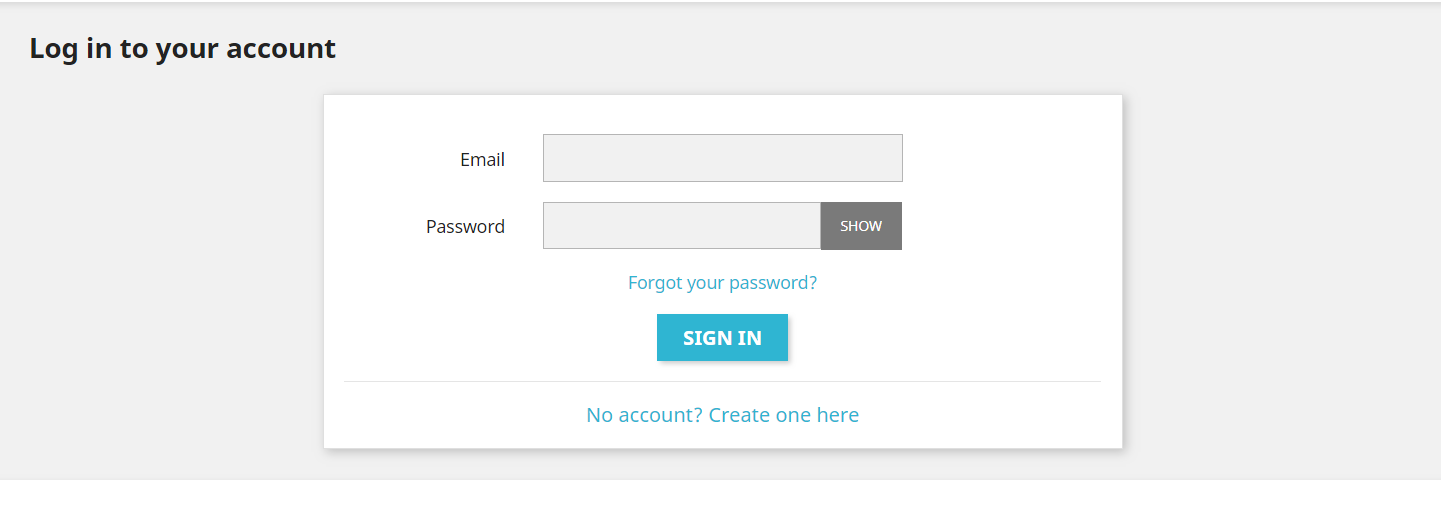
\includegraphics[height=2in]{/home/basedul/Documents/Report-writing-using-latex/HouseRentalManagementSystem/chapter-4/user-interface.png}
%		\caption{User Interface}
%		\label{fig:user-int} 
%\end{figure}
%\begin{figure}[H]
%		\centering
%		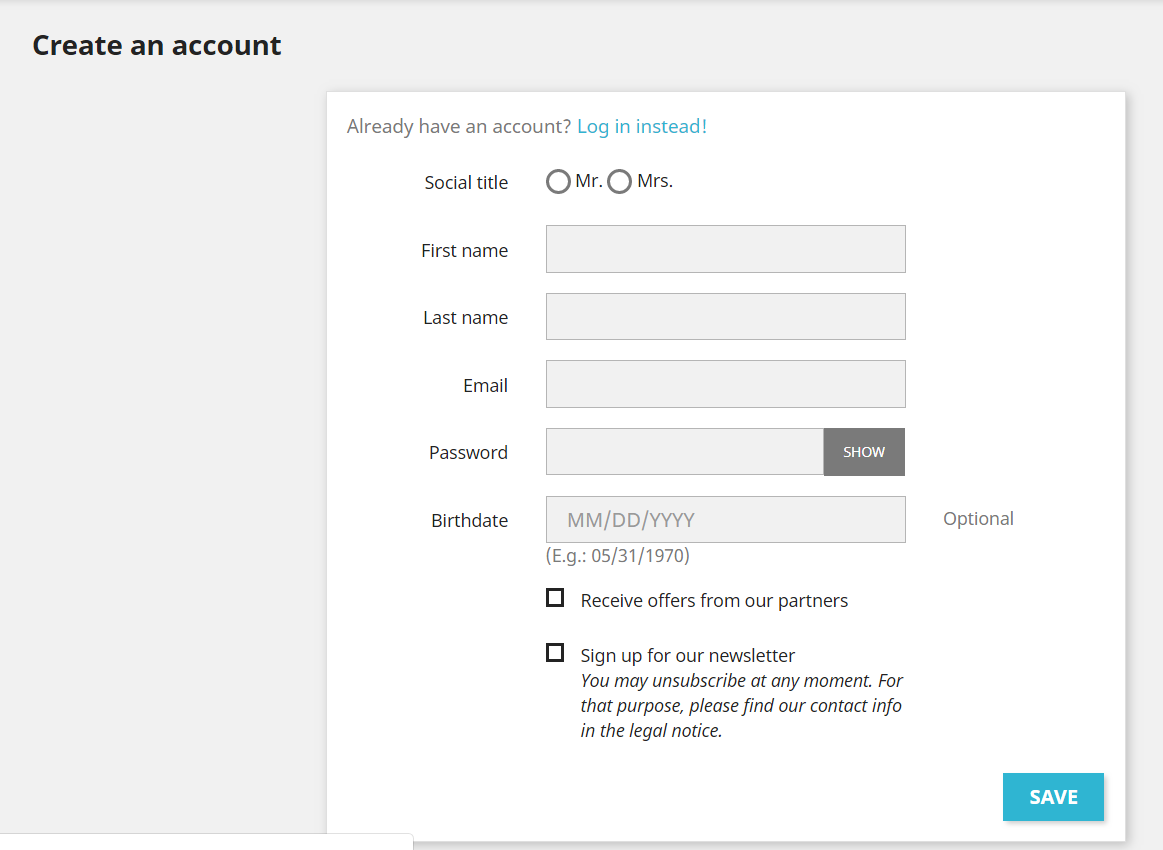
\includegraphics[height=3in]{/home/basedul/Documents/Report-writing-using-latex/HouseRentalManagementSystem/chapter-4/user-interface2.png}
%		%\caption{User Interface}
%		\label{fig:user-int2} 
%\end{figure}
%
\begin{figure}[H]
 \centering
\begin{subfigure}{0.5\textwidth}
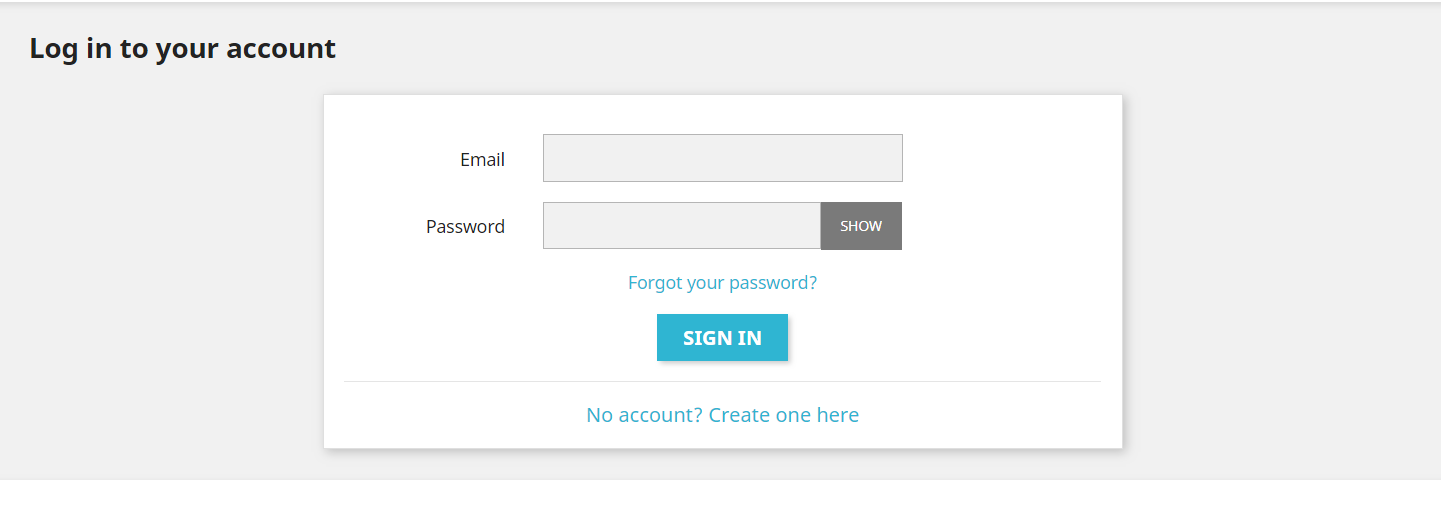
\includegraphics[width=1.2\linewidth, height=7cm]{/home/basedul/Documents/Report-writing-using-latex/HouseRentalManagementSystem/chapter-4/user-interface.png} 
%\caption{Caption1}
\label{fig:user-int}
\end{subfigure}
\begin{subfigure}{0.5\textwidth}
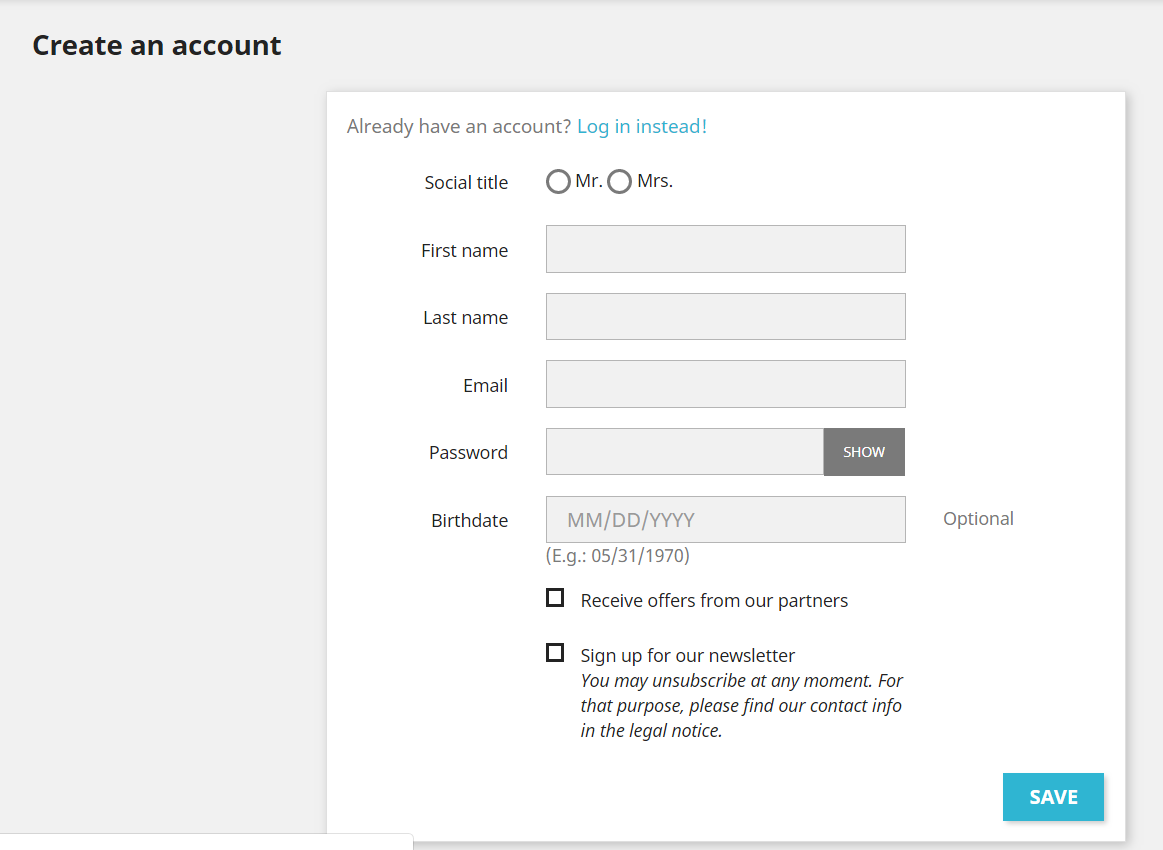
\includegraphics[width=1.2\linewidth, height=7cm]{/home/basedul/Documents/Report-writing-using-latex/HouseRentalManagementSystem/chapter-4/user-interface2.png}
%\caption{Caption 2}
\label{fig:subim2}
\end{subfigure}
 
\caption{\hspace{0.35em}User Interface}
\label{fig:user-info}
\end{figure}

	\subsection{Results of Search feature}
	\tab A search term\cite{Ref:18}, or search query, is the word or phrase someone enters into a search engine to search for on the internet. These can be single words or names, like [Yoast], or a combination of words, such as [buy robot vacuum cleaner], or even complete questions, like [how do I train my puppy?]. Note that each individual could phrase his or her query uniquely, so five people looking for the exact same thing may just use five completely different search terms. Moreover, search terms can contain spelling errors, numbers substituting words, or random word order, and still take someone where they need to be.\\While everyone entering a search term into a search engine is trying to find something, their intent can certainly differ. It’s important to be aware of this. Someone typing [how do I train my puppy?] into Google is looking for information, whereas someone who enters [Yoast] probably wants to navigate to Yoast.com. And someone looking for [buy robot vacuum cleaner] is, evidently, looking to buy a robot vacuum sometime in the near future.\\If the page someone clicks on in the search results doesn’t match their intent, they’re likely to bounce back and look for another page that does align with their purpose. So, you’ll understand that it’s important, as a site owner, to make sure people end up on a page that’s consistent with their expectations and what they’re trying to achieve!\\In fig-\ref{fig:search} as mentioned in the previous chapter of implementation we explained how one can opt for a choice of
priority. Based on the selected priority the results will vary in some extent.
\begin{figure}[H]
 \centering
\begin{subfigure}{0.5\textwidth}
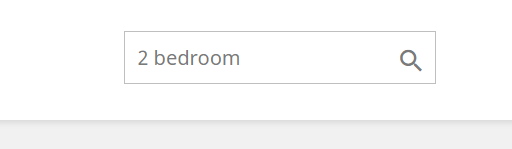
\includegraphics[width=0.9\linewidth, height=5cm]{/home/basedul/Documents/Report-writing-using-latex/HouseRentalManagementSystem/chapter-4/res-search-one.png} 
%\caption{Caption1}
\label{fig:search1}
\end{subfigure}
\begin{subfigure}{0.5\textwidth}
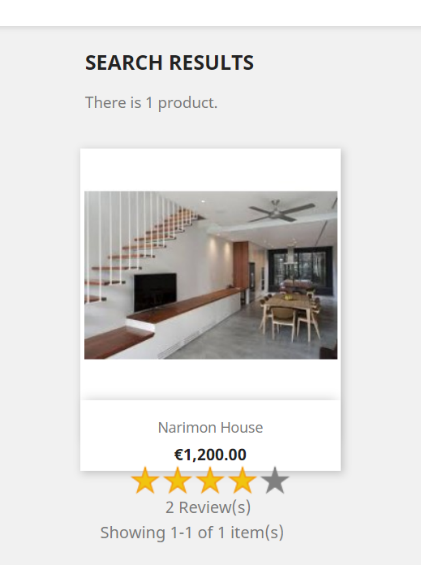
\includegraphics[width=1\linewidth, height=7cm]{/home/basedul/Documents/Report-writing-using-latex/HouseRentalManagementSystem/chapter-4/res-search-TWO.png}
%\caption{Caption 2}
\label{fig:hyuuua}
\end{subfigure}
 
\caption{\hspace{0.35em}Search User Interface}
\label{fig:search}
\end{figure}

	\subsection{Goggle Map}
		\tab Google Maps\cite{Ref:19} is a Web-based service that provides detailed information about geographical regions and sites around the world. In addition to conventional road maps, Google Maps offers aerial and satellite views of many places. In some cities, Google Maps offers street views comprising photographs taken from vehicles.\\Google Maps offers several services as part of the larger Web application, as follows.
		\begin{itemize}
			\item A route planner offers directions for drivers, bikers, walkers, and users of public transportation who want to take a trip from one specific location to another.
			\item The Google Maps application program interface (API) makes it possible for Web site administrators to embed Google Maps into a proprietary site such as a real estate guide or community service page.
			\item Google Maps for Mobile offers a location service for motorists that utilizes the Global Positioning System (GPS) location of the mobile device (if available) along with data from wireless and cellular networks.
			\item Google Street View enables users to view and navigate through horizontal and vertical panoramic street level images of various cities around the world.
			\item Supplemental services offer images of the moon, Mars, and the heavens for hobby astronomers.
		\end{itemize}
In fig-\ref{fig:map} the area shows the location of the user the user has provided the system while searching for rentals. Other the pointers show the results of the search based on area focusing the area Niketon.
Upon clicking the Details button attached with every rental shown in the box the user will be redirected
to page where not only the user can see the details of the rental including pictures but the user can also
search for the transport by manually providing the location as we have not integrated GPS system to
automatically extract the user location yet.
	\begin{figure}[H]
		\centering
		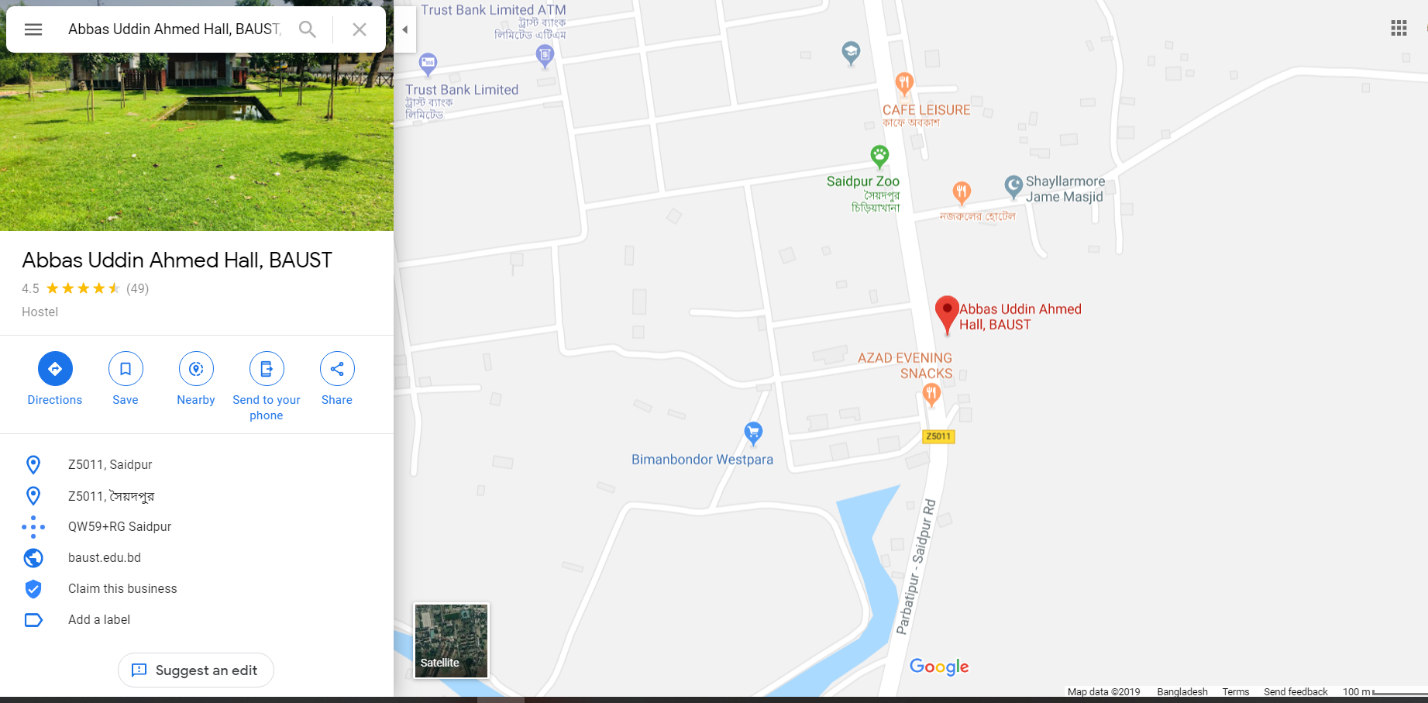
\includegraphics[height=2.5in]{/home/basedul/Documents/Report-writing-using-latex/HouseRentalManagementSystem/chapter-4/goggle-map.png}
		\caption{\hspace{0.35em}Architecture of House Rental Management System}
		\label{fig:map} 
	\end{figure}
	
	\subsection{Home page}
	\tab{In fig: \ref{fig:homepage} we try to show the homepage of our implementation. In homepage there are three types feature like House, Hotels, Cars. If we select houses, show us homes in different category like 2 beds, 3 beds, one kitchen and one bathroom etc. If rent seekers select a house then show the description of house and so that contact with rent seekers by contact number, this number is kept in description section. Finally, selected a house and also find the location of house. If landlord want to upload a house and house details, first of all landlord should have contact with admin and admin want to get the license of house and details of house after fulfill the condition between landlord and admin, house is uploaded and show our home page. In homepage also have a chatbox, by chatbox different types of user like landlord, rent seekers and govt. can contact with admin.	
	\begin{figure}[H]
 \centering
\begin{subfigure}{1.1\textwidth}
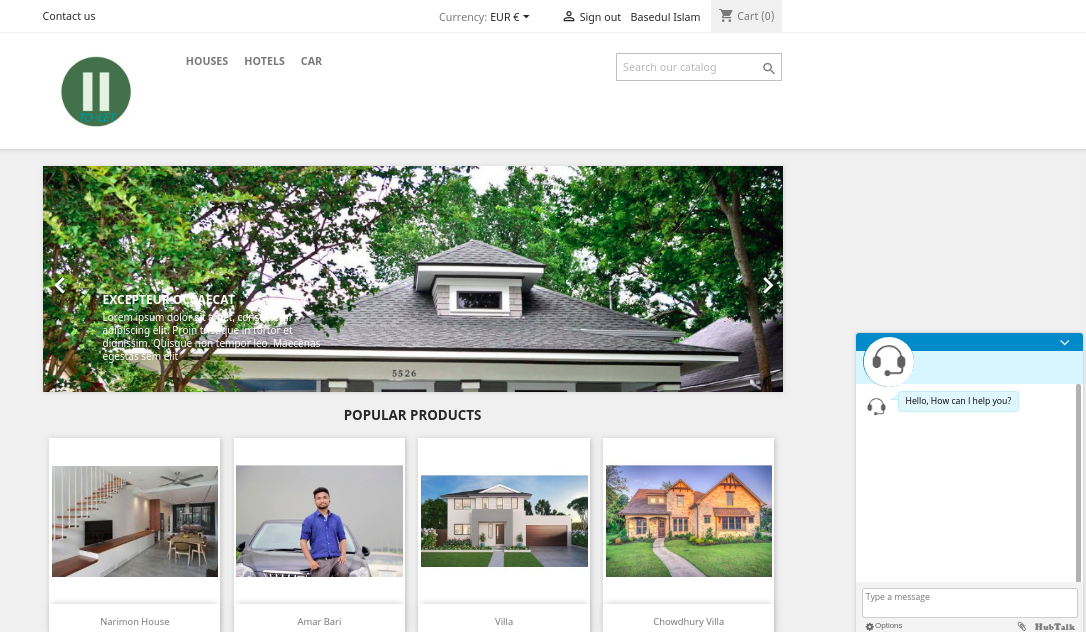
\includegraphics[width=0.9\linewidth, height=5cm]{/home/basedul/Documents/Report-writing-using-latex/HouseRentalManagementSystem/house-pik/home-page.png} 
%\caption{Caption1}
\label{fig:search1}
\end{subfigure}
\begin{subfigure}{1.1\textwidth}
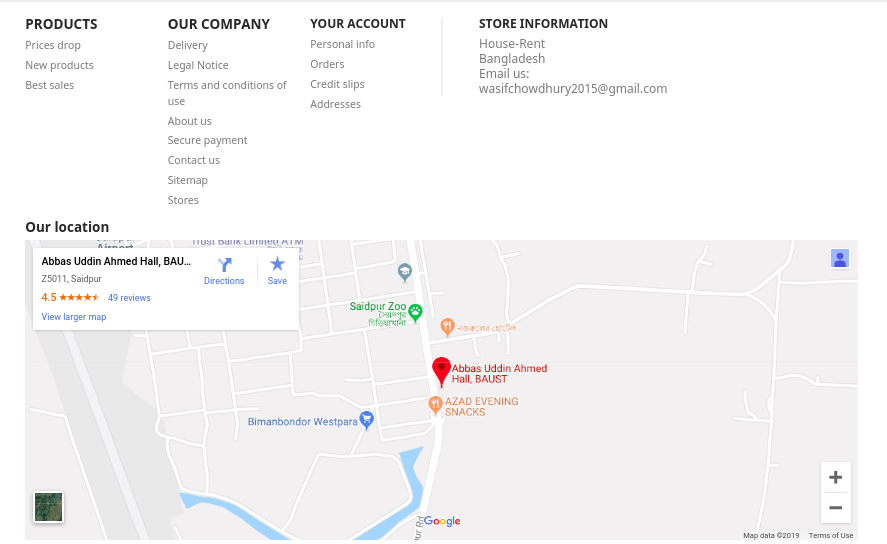
\includegraphics[width=0.9\linewidth, height=5cm]{/home/basedul/Documents/Report-writing-using-latex/HouseRentalManagementSystem/house-pik/underdown-homepage.png}
%\caption{Caption 2}
\label{fig:hyuuua}
\end{subfigure}
 
\caption{\hspace{0.35em}Homepage User Interface}
\label{fig:homepage}
\end{figure}


	\subsection{Chat box}
	\tab{In fig: \ref{fig:chat-box}, we see the chat box, that chat box is opened for all types of user for contact with user. If a landlord don't know how to upload his house in our website he/she can contact with us through this chat box and get a solution of it. If the agent found off line, they can still send a off line message to our agents.}
	\begin{figure}[H]
		\centering
		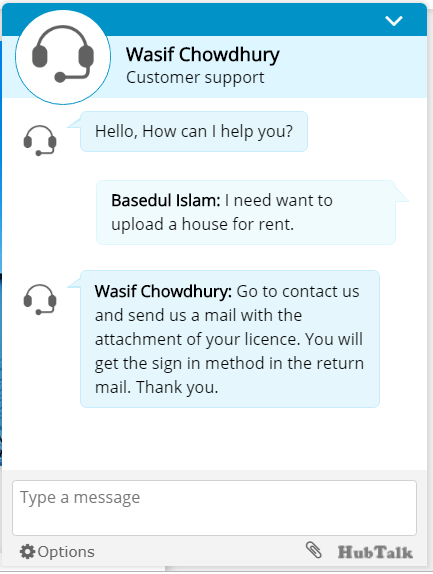
\includegraphics[height=3.5in]{/home/basedul/Documents/Report-writing-using-latex/HouseRentalManagementSystem/house-pik/chat-box.png}
		\caption{\hspace{0.35em}Chat box}
		\label{fig:chat-box} 
	\end{figure}
	
	\subsection{Contact between landlord \& admin}
	\tab{In fig: \ref{fig:con-ad}, By contact us window, any other users can contact with admin. This is the most important area for the landlords.From here a landlord need to contact with us to upload their house. First they need to send us a mail with a attachment of the license of their and a request of uploading their house.In return mail we will send them a specific e-mail and password by which they can access the house list and upload their house. As shown in fig: \ref{fig:pro-ad}.
	\begin{figure}[H]
		\centering
		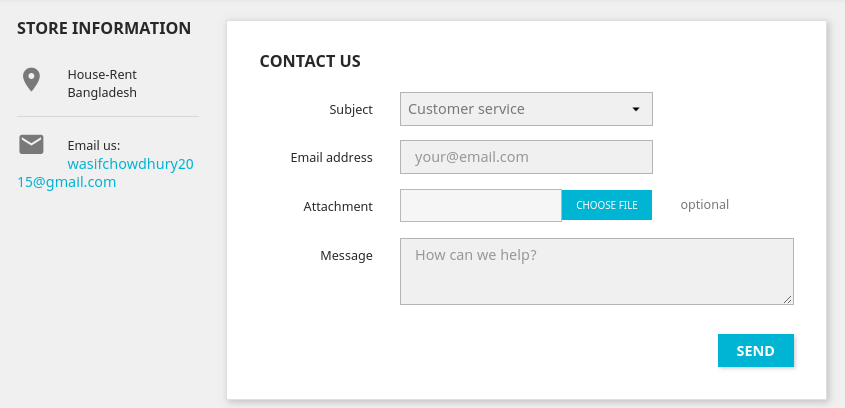
\includegraphics[height=2.5in]{/home/basedul/Documents/Report-writing-using-latex/HouseRentalManagementSystem/house-pik/contact-us.png}
		\caption{\hspace{0.35em}Contact Us}
		\label{fig:con-ad} 
	\end{figure}
	\begin{figure}[H]
		\centering
		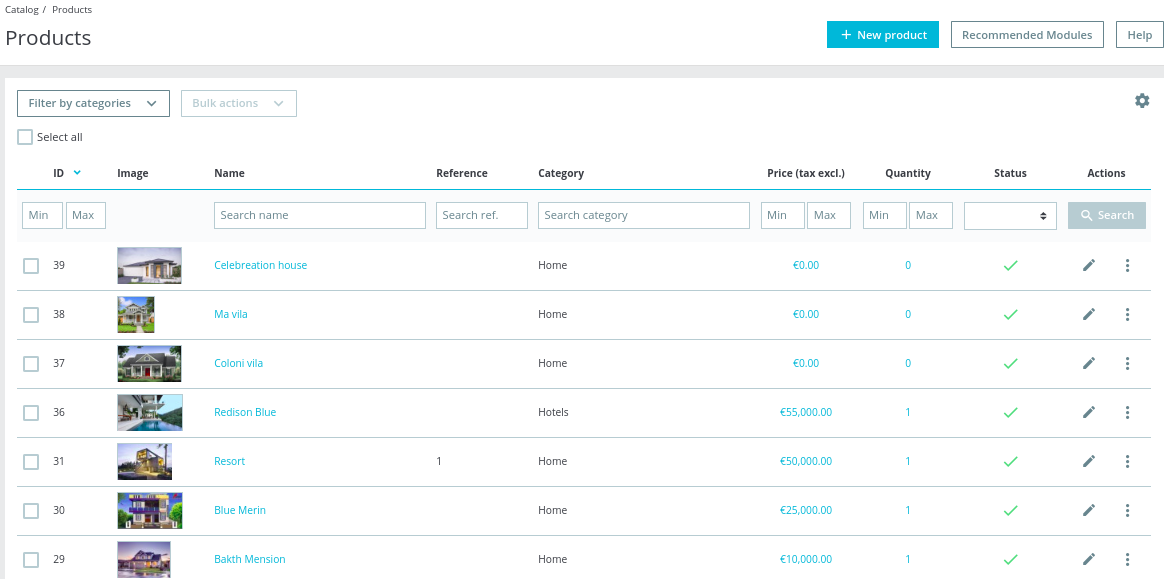
\includegraphics[height=3in]{/home/basedul/Documents/Report-writing-using-latex/HouseRentalManagementSystem/house-pik/product.png}
		\caption{\hspace{0.35em}House list \& upload}
		\label{fig:pro-ad} 
	\end{figure}
	
	\section{Government}
	{The Government can also be benefited by  this project. They can keep a track of everyone who is living where.This will help to reduce crime in our country and will also prevent terrorism in our country. The government will have a specific id given by the admin. As shown in fig: \ref{fig:cus-list}
	
	\begin{figure}[H]
		\centering
		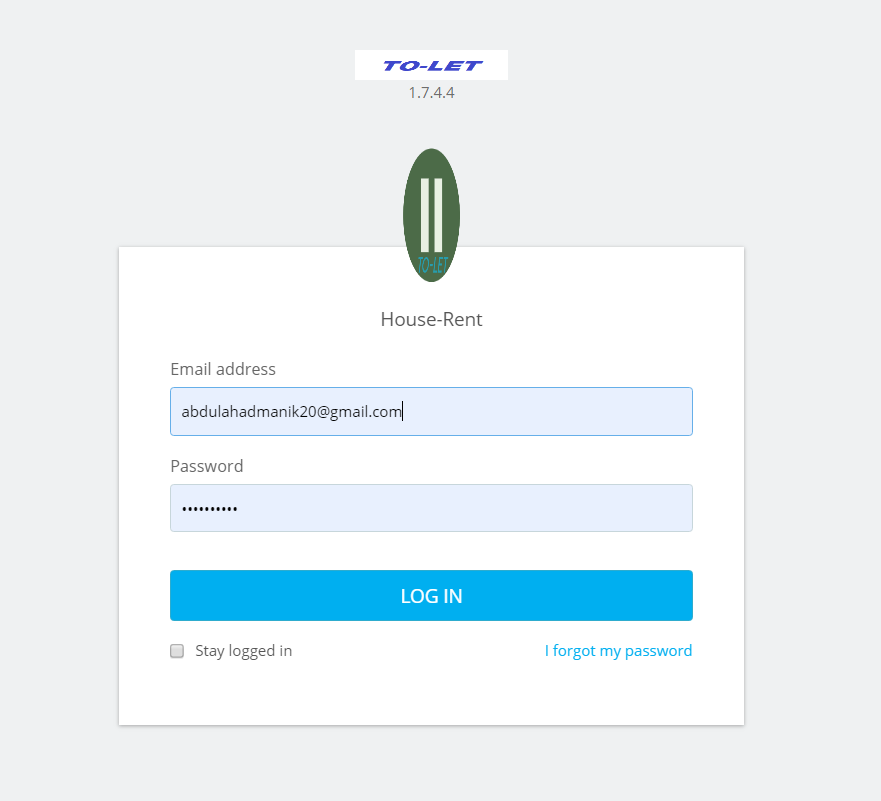
\includegraphics[height=3in]{/home/basedul/Documents/Report-writing-using-latex/HouseRentalManagementSystem/house-pik/wasif1.png}
		\caption{\hspace{0.35em} Government login}
		\label{fig:govt-login} 
	\end{figure}	
	
	\RaggedRight They can access the customer list and address from there.It will help them to keep an eye on someone who is suspicious.It will help to keep crime rate under control.
	\begin{figure}[H]
		\centering
		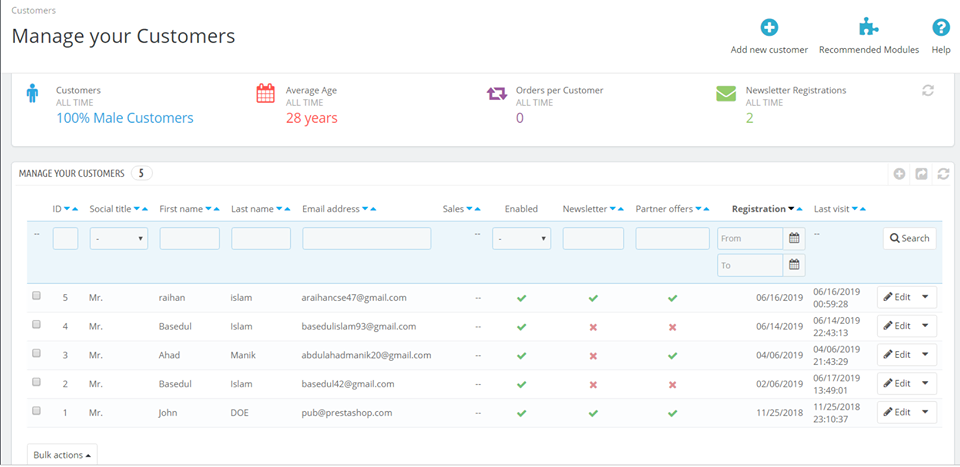
\includegraphics[height=3in]{/home/basedul/Documents/Report-writing-using-latex/HouseRentalManagementSystem/house-pik/wasif2.png}
		\caption{\hspace{0.35em} Customer list \& address}
		\label{fig:cus-list} 
	\end{figure}
	}
	\section{Test Case}
	\tab{A Test case\cite{Ref:20} is an automated test that addresses one objective of a test plan.\\A test case:
	\begin{itemize}
		\item Drives the application from the initial state to the state you want to test.
		\item Verifies that the actual state matches the expected (correct) state. Your QA department might use the term baseline to refer to this expected state. This stage is the heart of the test case.
		\item Cleans up the application, in preparation for the next test case, by undoing the steps performed in the first stage.
	\end{itemize}
	In order for a test case to function properly, the application must be in a stable state when the test case begins to execute. This stable state is called the base state. The recovery system is responsible for maintaining the base state in the event the application fails or crashes, either during the execution of a test cases or between test cases.\\Each test case is independent and should perform its own setup, driving the application to the state that you want to test, executing the test case, and then returning the application to the base state. The test case should not rely on the successful or unsuccessful completion of another test case, and the order in which the test case is executed should have no bearing on its outcome. If a test case relies on a prior test case to perform some setup actions, and an error causes the setup to fail or, worse yet, the application to crash, all subsequent test cases will fail because they cannot achieve the state where the test is designed to begin.\\A test case has a single purpose: a single test case should verify a single aspect of the application. When a test case designed in this manner passes or fails, it is easy to determine specifically what aspect of the target application is either working or not working.\\If a test case contains more than one objective, many outcomes are possible. Therefore, an exception may not point specifically to a single failure in the software under test but rather to several related function points. This makes debugging more difficult and time-consuming and leads to confusion in interpreting and quantifying results. The result is an overall lack of confidence in any statistics that might be generated. But there are techniques you can use to perform more than one verification in a test case.\\A Test cases a set of conditions or variables under which a tester will determine
whether a system under test satisfies requirements or works correctly. The process of
developing test cases can also help find problems in the requirements or design of an
application.\\Test cases were created to test adding, deleting, and editing both house items.
Specifically these test cases make certain that houses are stored and retrieved
from the database correctly. Test cases were also generated to perform boundary testing
on how many entries could be successfully added or updated. In addition, test cases where
created to verify the function of the compare class, which is used to validate input.	

\begin{table}[H]
\center
\renewcommand\arraystretch{0}
		\label{tab:Test}
\caption{\hspace{0.4em}Test Cases}
\vspace{0.2cm}
\begin{tabular}{M{2cm}|M{3cm}|M{3cm}|M{3cm}|M{1.5cm}N}
%Start
\hline
\textbf{Scenario} &
{\textbf{Test Cases}} & 
{\textbf{Expected Result}} & %
{\textbf{Test Result}} &
\textbf{Pass or Fail} & \\ [10pt]
\hline
\fontsize {10}{8}\fontfamily{ptm}\selectfont {} & 
\fontsize {10}{8}\fontfamily{ptm}\selectfont {Enter null in
mandatory fields.} & 
\fontsize {10}{8}\fontfamily{ptm}\selectfont {It should not do the
registration and
show error.} & 
\fontsize {10}{8}\fontfamily{ptm}\selectfont {It will show
message that please
fill out this field.} & 
\fontsize {10}{8}\fontfamily{ptm}\selectfont {Pass} &\\[30pt]
\cline{2-6}%next

\fontsize {10}{8}\fontfamily{ptm}\selectfont {Registration} & 
\fontsize {10}{8}\fontfamily{ptm}\selectfont {Enter incorrect data} & 
\fontsize {10}{8}\fontfamily{ptm}\selectfont {It should not do the
registration and
show error.} & 
\fontsize {10}{8}\fontfamily{ptm}\selectfont {Email: Please enter
an email.
Password:
Password.
do not match} & 
\fontsize {10}{8}\fontfamily{ptm}\selectfont {Pass} &\\[35pt]
\cline{2-6}%next

\fontsize {10}{8}\fontfamily{ptm}\selectfont {} & 
\fontsize {10}{8}\fontfamily{ptm}\selectfont {Enter correct data of
all required field} & 
\fontsize {10}{8}\fontfamily{ptm}\selectfont {It should lead to
successfully
registration} & 
\fontsize {10}{8}\fontfamily{ptm}\selectfont {It will show the
message of
successfully
registrattion} & 
\fontsize {10}{8}\fontfamily{ptm}\selectfont {Pass} &\\[40pt]
\hline%next

\fontsize {10}{8}\fontfamily{ptm}\selectfont {} & 
\fontsize {10}{8}\fontfamily{ptm}\selectfont {Enter null email or
password.} & 
\fontsize {10}{8}\fontfamily{ptm}\selectfont {It should not do the
login and show
error.} & 
\fontsize {10}{8}\fontfamily{ptm}\selectfont {It will show
message that please
fill out this field.} & 
\fontsize {10}{8}\fontfamily{ptm}\selectfont {Pass} &\\[33pt]
\cline{2-6}%next

\fontsize {10}{8}\fontfamily{ptm}\selectfont {Login} & 
\fontsize {10}{8}\fontfamily{ptm}\selectfont {Enter wrong data of
email or password.} & 
\fontsize {10}{8}\fontfamily{ptm}\selectfont {It should not do the
login and show
error.} & 
\fontsize {10}{8}\fontfamily{ptm}\selectfont {It will show message
that please enter an
email or your email
address or password
are not correct..} & 
\fontsize {10}{8}\fontfamily{ptm}\selectfont {Pass} &\\[55pt]
\cline{2-6}%next

\fontsize {10}{8}\fontfamily{ptm}\selectfont {} & 
\fontsize {10}{8}\fontfamily{ptm}\selectfont {Enter correct data of
email or password.} & 
\fontsize {10}{8}\fontfamily{ptm}\selectfont {It should let do the
login.} & 
\fontsize {10}{8}\fontfamily{ptm}\selectfont {It will redirect to
your all purchased
products} & 
\fontsize {10}{8}\fontfamily{ptm}\selectfont {Pass} &\\[33pt]
\hline%next

\fontsize {10}{8}\fontfamily{ptm}\selectfont {} & 
\fontsize {10}{8}\fontfamily{ptm}\selectfont {Enter null in
mandatory fields.} & 
\fontsize {10}{8}\fontfamily{ptm}\selectfont {It should not do the
update and show
error.} & 
\fontsize {10}{8}\fontfamily{ptm}\selectfont {It will show
message that please
fill out this field.} & 
\fontsize {10}{8}\fontfamily{ptm}\selectfont {Pass} &\\[33pt]
\cline{2-6}%next

\fontsize {10}{8}\fontfamily{ptm}\selectfont {Update
password} & 
\fontsize {10}{8}\fontfamily{ptm}\selectfont {Enter incorrect data} & 
\fontsize {10}{8}\fontfamily{ptm}\selectfont {It should not do the
update and show
error.} & 
\fontsize {10}{8}\fontfamily{ptm}\selectfont {It will show the
message that the old
password do not
match.} & 
\fontsize {10}{8}\fontfamily{ptm}\selectfont {Pass} &\\[42pt]
\cline{2-6}%next

\fontsize {10}{8}\fontfamily{ptm}\selectfont {} & 
\fontsize {10}{8}\fontfamily{ptm}\selectfont {Enter correct data of
all required field.} & 
\fontsize {10}{8}\fontfamily{ptm}\selectfont {It should let do
registration.} & 
\fontsize {10}{8}\fontfamily{ptm}\selectfont {It will show the
message that
password
successfully
updated.} & 
\fontsize {10}{8}\fontfamily{ptm}\selectfont {Pass} &\\[40pt]
\hline%next

\fontsize {10}{8}\fontfamily{ptm}\selectfont {Search
House} & 
\fontsize {10}{8}\fontfamily{ptm}\selectfont {Enter null or
incorrect data in
search fields.} & 
\fontsize {10}{8}\fontfamily{ptm}\selectfont {It will not search
house} & 
\fontsize {10}{8}\fontfamily{ptm}\selectfont {It will show the
message that there
was no search
results!} & 
\fontsize {10}{8}\fontfamily{ptm}\selectfont {Pass} &\\[40pt]
\cline{2-6}%next


\fontsize {10}{8}\fontfamily{ptm}\selectfont {} & 
\fontsize {10}{8}\fontfamily{ptm}\selectfont {Enter correct data in
Search fields.} & 
\fontsize {10}{8}\fontfamily{ptm}\selectfont {It should search
houses depending the
keywords.} & 
\fontsize {10}{8}\fontfamily{ptm}\selectfont {It will display the
houses regarding the
keywords.} & 
\fontsize {10}{8}\fontfamily{ptm}\selectfont {Pass} &\\[33pt]
\hline%next


\fontsize {10}{8}\fontfamily{ptm}\selectfont {Comment
on house} & 
\fontsize {10}{8}\fontfamily{ptm}\selectfont {Enter non ASCII
character.} & 
\fontsize {10}{8}\fontfamily{ptm}\selectfont {It will not let to
comment} & 
\fontsize {10}{8}\fontfamily{ptm}\selectfont {It will show error as
unsupported
character.} & 
\fontsize {10}{8}\fontfamily{ptm}\selectfont {Pass} &\\[30pt]
\cline{2-6}%next


\fontsize {10}{8}\fontfamily{ptm}\selectfont {} & 
\fontsize {10}{8}\fontfamily{ptm}\selectfont {Enter ASCII
character.} & 
\fontsize {10}{8}\fontfamily{ptm}\selectfont {It will lead a
successful comment.} & 
\fontsize {10}{8}\fontfamily{ptm}\selectfont {It will view the
succession of a
comment.} & 
\fontsize {10}{8}\fontfamily{ptm}\selectfont {Pass} &\\[25pt]
\hline%next
%\multirow{3}{1.5cm}[-1.7em]{\begin{flushleft}
%\centering Registration
%\end{flushleft}} &
%
%\multicolumn{2}{M{3.5cm}|}{\begin{flushleft}
%Enter null in
%mandatory fields.
%\end{flushleft}} &
%\multicolumn{2}{M{3.5cm}|}{\begin{flushleft}
%It should not do the
%registration
%and show error.
%\end{flushleft}} & %
%\multicolumn{2}{M{3.5cm}|}{\begin{flushleft}
%It will show message
%that please fill out this
%field.
%\end{flushleft}} &
%Pass & \\[0pt]\cline{2-9} &
%\multicolumn{2}{M{3.5cm}|}{\begin{flushleft}
%Enter incorrect data
%\end{flushleft}} & 
%\multicolumn{2}{M{3.5cm}|}{\begin{flushleft}
%It should not do the
%registration and show error.
%\end{flushleft}} & 
%\multicolumn{2}{M{3.5cm}|}{\begin{flushleft}
%Email: Please enter an email.
%\linebreak
%Password: Password.\linebreak
%do not match\end{flushleft}} & Pass\\[25pt]\cline{2-9}& 
%\multicolumn{2}{M{3.5cm}|}{\begin{flushleft}
%Enter correct data of all 
%required field
%\end{flushleft}} & 
%\multicolumn{2}{M{3.5cm}|}{\begin{flushleft}
%It should lead to successfully registration
%\end{flushleft}} & 
%\multicolumn{2}{M{3.5cm}|}{\begin{flushleft}
%It will show the message of successfully registrattion
%\end{flushleft}} & Pass\\ [25pt]
%\hline
%\multirow{3}{1.5cm}[-1.5em]{\centering Login} &
%
%\multicolumn{2}{M{3.5cm}|}{\begin{flushleft}
%Enter null email or
%password.
%\end{flushleft}} &
%\multicolumn{2}{M{3.5cm}|}{\begin{flushleft}
%It should not do the
%login and show error.
%\end{flushleft}
%} & %
%\multicolumn{2}{M{3.5cm}|}{\begin{flushleft}
%It will show message that please fill out this field.
%\end{flushleft}} &
%Pass & \\[0pt]\cline{2-9} &
%\multicolumn{2}{M{3.5cm}|}{\begin{flushleft}
%Enter wrong data of
%email or password.
%\end{flushleft}} & 
%\multicolumn{2}{M{3.5cm}|}{\begin{flushleft}
%It should not do the login and show error.
%\end{flushleft}} & 
%\multicolumn{2}{M{3.5cm}|}{\begin{flushleft}
%It will show message that please enter an email or your email address or password are not correct.
%\end{flushleft}
%} & Pass\\[25pt]\cline{2-9}& 
%\multicolumn{2}{M{3.5cm}|}{\begin{flushleft}
%Enter correct data of
%email or password.
%\end{flushleft}} & 
%\multicolumn{2}{M{3.5cm}|}{\begin{flushleft}
%It should let do the login.
%\end{flushleft}
%} & 
%\multicolumn{2}{M{3.5cm}|}{\begin{flushleft}
%It will redirect to your all purchased products
%\end{flushleft}
%} & Pass\\ [25pt]
%\hline%End
%\hline%Start
%\multirow{3}{1.5cm}[-1.5em]{\centering Update password
%} &
%
%\multicolumn{2}{M{3.5cm}|}{\begin{flushleft}
%Enter null in
%mandatory fields.
%\end{flushleft}
%} &
%\multicolumn{2}{M{3.5cm}|}{\begin{flushleft}
%It should not do the update
%and show error.
%\end{flushleft}} & %
%\multicolumn{2}{M{3.5cm}|}{\begin{flushleft}
%It will show message that please fill out this field.
%\end{flushleft}} &
%Pass & \\[0pt]\cline{2-9} &
%\multicolumn{2}{M{3.5cm}|}{\begin{flushleft}
%Enter incorrect data
%\end{flushleft}} & 
%\multicolumn{2}{M{3.5cm}|}{\begin{flushleft}
%It should not do the update
%and show error.
%\end{flushleft}} & 
%\multicolumn{2}{M{3.5cm}|}{\begin{flushleft}
%It will show the message that the old password do not match.
%\end{flushleft}
%} & Pass\\[25pt]\cline{2-9}& 
%\multicolumn{2}{M{3.5cm}|}{\begin{flushleft}
%Enter correct data of all
%required field.
%\end{flushleft}} & 
%\multicolumn{2}{M{3.5cm}|}{\begin{flushleft}
%It should let do
%registration.
%\end{flushleft}} & 
%
%\multicolumn{2}{M{3.5cm}|}{\begin{flushleft}
%It will show the message that password successfully updated.
%\end{flushleft}
%} & Pass\\ [25pt]
%\hline%End
%\hline%Start
%\multirow{2}{1.5cm}[-1.5em]{\centering Search Food
%} &
%
%\multicolumn{2}{M{3.5cm}|}{\begin{flushleft}
%Enter null or incorrect data in search fields.
%\end{flushleft}
%} &
%\multicolumn{2}{M{3.5cm}|}{\begin{flushleft}
%It will not search food
%\end{flushleft}} & %
%\multicolumn{2}{M{3.5cm}|}{\begin{flushleft}
%It will show the message that there was no search results!
%\end{flushleft}} &
%Pass & \\[0pt]\cline{2-9} &
%\multicolumn{2}{M{3.5cm}|}{\begin{flushleft}
%Enter correct data in
%Search fields.
%\end{flushleft}} & 
%\multicolumn{2}{M{3.5cm}|}{\begin{flushleft}
%It should search foods depending the keywords.
%\end{flushleft}} & 
%\multicolumn{2}{M{3.5cm}|}{\begin{flushleft}
%It will display the foods regarding the keywords.
%\end{flushleft}
%} & Pass\\[25pt]
%\hline%End
%\hline%Start
%\multirow{2}{1.5cm}[-1.5em]{\centering Comment Food
%} &
%
%\multicolumn{2}{M{3.5cm}|}{\begin{flushleft}
%Enter non ASCII character.
%\end{flushleft}} &
%\multicolumn{2}{M{3.5cm}|}{\begin{flushleft}
%It will not let to comment
%\end{flushleft}
%} & %
%\multicolumn{2}{M{3.5cm}|}{\begin{flushleft}
%It will show error as unsupported character.
%\end{flushleft}} &
%Pass & \\[0pt]\cline{2-9} &
%\multicolumn{2}{M{3.5cm}|}{\begin{flushleft}
%Enter ASCII character.
%\end{flushleft}} & 
%\multicolumn{2}{M{3.5cm}|}{\begin{flushleft}
%It will lead a successful comment.
%\end{flushleft}} & 
%\multicolumn{2}{M{3.5cm}|}{\begin{flushleft}
%It will view the succession of a comment.
%\end{flushleft}
%} & Pass\\[25pt]
%\hline%End

\end{tabular}
\end{table}
%
%\begin{table}[H]
%\renewcommand\arraystretch{0}
%\captionsetup{labelformat=empty}
%\caption[]{ }
%\vspace{0.2cm}
%
%\begin{tabular}{M{2.5cm}|M{4cm}|M{4cm}|M{4cm}|M{4cm}|M{4cm}|M{4cm}|M{1cm}N}
%%Start
%\hline
%\textbf{Scenario} &
%\multicolumn{2}{M{3.5cm}|}{\textbf{Test Cases}} & 
%\multicolumn{2}{M{3.5cm}|}{\textbf{Expected Result}} & %
%\multicolumn{2}{M{3.5cm}|}{\textbf{Test Result}} &
%\textbf{Pass or Fail} & \\ [25pt]

%\hline%Start
%\multirow{3}{1.5cm}[-1.5em]{\centering Registration} &
%
%\multicolumn{2}{M{3.5cm}|}{\begin{flushleft}
%Enter null in
%mandatory fields.
%\end{flushleft}} &
%\multicolumn{2}{M{3.5cm}|}{\begin{flushleft}
%It should not do the
%registration
%and show error.
%\end{flushleft}} & %
%\multicolumn{2}{M{3.5cm}|}{\begin{flushleft}
%It will show message
%that please fill out this
%field.
%\end{flushleft}} &
%Pass & \\[0pt]\cline{2-9} &
%\multicolumn{2}{M{3.5cm}|}{\begin{flushleft}
%Enter incorrect data
%\end{flushleft}} & 
%\multicolumn{2}{M{3.5cm}|}{\begin{flushleft}
%It should not do the
%registration and show error.
%\end{flushleft}} & 
%\multicolumn{2}{M{3.5cm}|}{\begin{flushleft}
%Email: Please enter an email.
%\linebreak
%Password: Password.\linebreak
%do not match\end{flushleft}} & Pass\\[25pt]\cline{2-9}& 
%\multicolumn{2}{M{3.5cm}|}{\begin{flushleft}
%Enter correct data of all 
%required field
%\end{flushleft}} & 
%\multicolumn{2}{M{3.5cm}|}{\begin{flushleft}
%It should lead to successfully registration
%\end{flushleft}} & 
%\multicolumn{2}{M{3.5cm}|}{\begin{flushleft}
%It will show the message of successfully registrattion
%\end{flushleft}} & Pass\\ [25pt]
%\hline
%%End
%\hline%Start
%\multirow{3}{1.5cm}[-1.5em]{\centering Login} &
%
%\multicolumn{2}{M{3.5cm}|}{\begin{flushleft}
%Enter null email or
%password.
%\end{flushleft}} &
%\multicolumn{2}{M{3.5cm}|}{\begin{flushleft}
%It should not do the
%login and show error.
%\end{flushleft}
%} & %
%\multicolumn{2}{M{3.5cm}|}{\begin{flushleft}
%It will show message that please fill out this field.
%\end{flushleft}} &
%Pass & \\[0pt]\cline{2-9} &
%\multicolumn{2}{M{3.5cm}|}{\begin{flushleft}
%Enter wrong data of
%email or password.
%\end{flushleft}} & 
%\multicolumn{2}{M{3.5cm}|}{\begin{flushleft}
%It should not do the login and show error.
%\end{flushleft}} & 
%\multicolumn{2}{M{3.5cm}|}{\begin{flushleft}
%It will show message that please enter an email or your email address or password are not correct.
%\end{flushleft}
%} & Pass\\[25pt]\cline{2-9}& 
%\multicolumn{2}{M{3.5cm}|}{\begin{flushleft}
%Enter correct data of
%email or password.
%\end{flushleft}} & 
%\multicolumn{2}{M{3.5cm}|}{\begin{flushleft}
%It should let do the login.
%\end{flushleft}
%} & 
%\multicolumn{2}{M{3.5cm}|}{\begin{flushleft}
%It will redirect to your all purchased products
%\end{flushleft}
%} & Pass\\ [25pt]
%\hline%End

%\multirow{3}{2cm}[-1.5em]{\centering Update password
%} &
%
%\multicolumn{2}{M{3.5cm}|}{\begin{flushleft}
%Enter null in
%mandatory fields.
%\end{flushleft}
%} &
%\multicolumn{2}{M{3.5cm}|}{\begin{flushleft}
%It should not do the update
%and show error.
%\end{flushleft}} & %
%\multicolumn{2}{M{3.5cm}|}{\begin{flushleft}
%It will show message that please fill out this field.
%\end{flushleft}} &
%Pass & \\[0pt]\cline{2-9} &
%\multicolumn{2}{M{3.5cm}|}{\begin{flushleft}
%Enter incorrect data
%\end{flushleft}} & 
%\multicolumn{2}{M{3.5cm}|}{\begin{flushleft}
%It should not do the update
%and show error.
%\end{flushleft}} & 
%\multicolumn{2}{M{3.5cm}|}{\begin{flushleft}
%It will show the message that the old password do not match.
%\end{flushleft}
%} & Pass\\[25pt]\cline{2-9}& 
%\multicolumn{2}{M{3.5cm}|}{\begin{flushleft}
%Enter correct data of all
%required field.
%\end{flushleft}} & 
%\multicolumn{2}{M{3.5cm}|}{\begin{flushleft}
%It should let do
%registration.
%\end{flushleft}} & 
%
%\multicolumn{2}{M{3.5cm}|}{\begin{flushleft}
%It will show the message that password successfully updated.
%\end{flushleft}
%} & Pass\\ [25pt]
%\hline%End
%\multirow{2}{1.5cm}[-1.5em]{\centering Search Food
%} &
%
%\multicolumn{2}{M{3.5cm}|}{\begin{flushleft}
%Enter null or incorrect data in search fields.
%\end{flushleft}
%} &
%\multicolumn{2}{M{3.5cm}|}{\begin{flushleft}
%It will not search food
%\end{flushleft}} & %
%\multicolumn{2}{M{3.5cm}|}{\begin{flushleft}
%It will show the message that there was no search results!
%\end{flushleft}} &
%Pass & \\[0pt]\cline{2-9} &
%\multicolumn{2}{M{3.5cm}|}{\begin{flushleft}
%Enter correct data in
%Search fields.
%\end{flushleft}} & 
%\multicolumn{2}{M{3.5cm}|}{\begin{flushleft}
%It should search foods depending the keywords.
%\end{flushleft}} & 
%\multicolumn{2}{M{3.5cm}|}{\begin{flushleft}
%It will display the foods regarding the keywords.
%\end{flushleft}
%} & Pass\\[25pt]
%\hline%End
%\multirow{2}{1.5cm}[-1.5em]{\centering Comment Food
%} &
%
%\multicolumn{2}{M{3.5cm}|}{\begin{flushleft}
%Enter non ASCII character.
%\end{flushleft}} &
%\multicolumn{2}{M{3.5cm}|}{\begin{flushleft}
%It will not let to comment
%\end{flushleft}
%} & %
%\multicolumn{2}{M{3.5cm}|}{\begin{flushleft}
%It will show error as unsupported character.
%\end{flushleft}} &
%Pass & \\[0pt]\cline{2-9} &
%\multicolumn{2}{M{3.5cm}|}{\begin{flushleft}
%Enter ASCII character.
%\end{flushleft}} & 
%\multicolumn{2}{M{3.5cm}|}{\begin{flushleft}
%It will lead a successful comment.
%\end{flushleft}} & 
%\multicolumn{2}{M{3.5cm}|}{\begin{flushleft}
%It will view the succession of a comment.
%\end{flushleft}
%} & Pass\\[25pt]
%\hline%End
%
%\end{tabular}
%\end{table}
	}	
		
	\begin{comment}		
		
	\begin{comment}
	\section{Introduction}
	\tab This project has been designed using numerous diagrammatic techniques. Recall from Section \ref{fig:uml}, that
the most general modeling language to describe both the structure and behavior of a software system
is Unified Modeling language (UML).
Use case diagrams have already been used in the requirements analysis as a way to graphically
overview the order process within the application. Other diagrams from the UML family are used in the
design stage to show the structure and behavior of numerous sophisticated design feature.
\section{Component Diagram}
\tab A component diagram is part of UML and its main purpose is to show the structural relationship
between components in the application. A component diagram is useful for this system as it shows the
higher architecture, as shown in figure \ref{fig:comdia}
\begin{figure}[H]
		\centering
		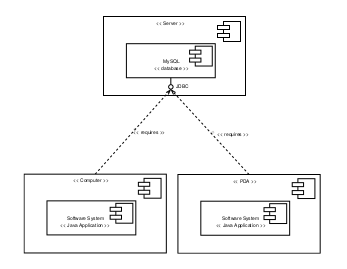
\includegraphics[height=3in]{/home/basedul/Documents/Report-writing-using-latex/ResturentManagementSystemReport/comdia.png}
		\caption{Component diagram showing the higher level architecture of the system.}
		\label{fig:comdia} 
	\end{figure}
	
\subsection{Data Storage}
	The Asian restaurant management application will be built around the data storage technique therefore choosing
the most appropriate persistent 1 data storage is critical to a successful project and we can assume a flat
file storage approach is inadequate. The two most popular types of persistent data storage available
are relational database management system (RDBMS) and extensible markup language (XML)
\subsubsection{Relational Database Management System (RDBMS)}
	\label{Rel:RDBMS}
	A relational database management system (RDBMS) is a database managed system based around a
relational model and are the corner stone’s to many software systems including web based systems.\\
RDBMS are one of the most popular data storage methods out in the market and offer many advantages
including:\\
\begin{itemize}
	\item Fast data extraction using structured query language (SQL).
	\item Good management of data and security through the management system.
	\item Good level of data consistency.
	\item Advanced features including functions and triggers.
	\item Requirement of a data model to be developed; leading to long term cost effectiveness. 
\end{itemize}
In industry, there are numerous expensive highly functional RDMBSs including Oracle and SQLServer
that are very popular and offer technical support. However, there are also numerous open-source solutions with many adjudged to be as good or better and are becoming even more popular with small
scale software systems.
\subsubsection{Extensible Markup Language (XML)}
	XML is a markup language that was designed to transport and store data and is another example of
a persistent data storage technique. However, it is not a predefined language thus all tags must be
defined and due to its hierarchically data structure all elements must be promoted or demoted.
XML could be used in two different ways in data storage; storing the XML documents within a
database or having the XML documents as the fundamental unit of storage. In both cases the XML
can be queried using either XPATH or XQUERY which are query languages for extracting data from
XML documents.
\subsubsection{Storage Method Chosen}
	The main difference between XML and RDBMS is that XML is hierarchical and RDBMS is relational.
As restaurant data can be best represented in a hierarchical way one would believe that XML would be
the best approach but it’s not always that straight forward. SQL is an extremely flexible and robust querying language and for the queries required and the type of software system begin designed, it was
concluded that RDBMS would be the best storage method.
The next choice was to decide on the type of RDBMS to use. As discussed there are many open
source RDBMSs available for us to choose from and for the main reason of experience, MySQL was the
preferred option. Figure \ref{fig:compari} shows just how competitive the performances of different RDBMSs are.
\begin{figure}[H]
		\centering
		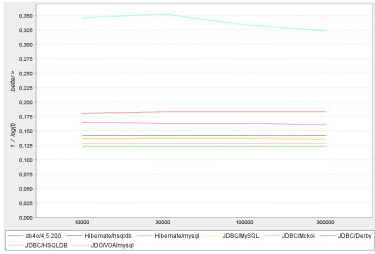
\includegraphics[height=4in]{/home/basedul/Documents/Report-writing-using-latex/ResturentManagementSystemReport/compari.png}
		\caption{Database comparison diagram \cite{Ref:6}}
		\label{fig:compari} 
	\end{figure}
\subsubsection{Normalisation}
Normalisation comes in many forms ranging from first normal form to sixth normal form. The nor-
malisation of a database is a systematic way to free the database of undesirable characteristics where
inserts, updates and deletions of data could lead to the loss of data integrity. The greater the normal
form, the greater the data integrity of the database.\\
The database in this system was designed to be in Boyce-Codd normal form which is a slightly
stronger version of the third normal form. For the database to be in Boyce-Codd normal form, it had
to pass for all previous normal forms as well as Boyce-Codd normal form.\\
A well designed database will normally abide by the first, second and third normal forms as they
are the basics to a well structured relational database. According to Horsforth School [17], the first
three normal forms can be defined as:
\begin{itemize}
	\item Every attribute is atomic or single valued therefore there are no repeating fields.
	\item All attributes not part of the primary key must be dependent on the full key.
	\item There must be no transitive determinants, or each attribute that is not part of
the key must be determined only by the key.
\end{itemize}
Finally for the database to be in the desired Boyce-Codd normal form, all tables must abide by the
first, second and third normal forms and must not have any determinants that are not candidate keys
for the table.
\end{commment}
\begin{comment}
\subsubsection{Entity Relationship Diagram}
	\label{sec:entity}
An entity relationship (ER) diagram is a modeling language used to represent a type of semantic
data model of a system. The ER diagrams are often used to represent a relational database and its
requirements in a top-down fashion usually defined as the database schema. The database schema for
this database has been split into two ER diagrams (Figures \ref{fig:entityone} and \ref{fig:entitytwo}).
Figure \ref{fig:entityone} graphically shows the objects and their relationships that are contained within a meal.
The meal object will be made of at least two ingredients that can be either a normal ingredient or
a prepared ingredient. Note, a prepared ingredient is a collection of ingredients used to either group
commonly used ingredients or to group optional ingredients. Each ingredient will have a default and
manual measurement with the default measurement entered on input of the ingredient and the manual
measurement entered if the meal ingredient link requires a different amount.
Also, each ingredient will be part of a generic ingredient object as there are many ingredients that
are the same item but packaged in a different way at a different price. This allows the database to be in
Boyce-Codd normalised state. An example of this would be the drink Coca-Cola which can be bought
by bottle, can or drought, thus are the same item but packaged differently at a different price and
amount. Finally each ingredient and prepared ingredient can be part of a category allowing optional
ingredients to be interchanged with other ingredients in the same category.
Figure \ref{fig:entitytwo} graphically shows the relationships for the menu, order and offer objects. The menu
consists of a date time relationship that provides the intervals to when the menu is active and a menu
section relationship that contains the color variables and items under that particular menu section.
The order consists of one to many suborders with the suborder consisting of one to many items.
The order stores all the ingredients within each item and also the replaced ingredient if that optional
ingredient was replaced.
The offer consists of a date time relationship that provides the intervals to when the offer is active
and a offer section relationship that contains the sets required by the offer.
\begin{figure}[H]
		\centering
		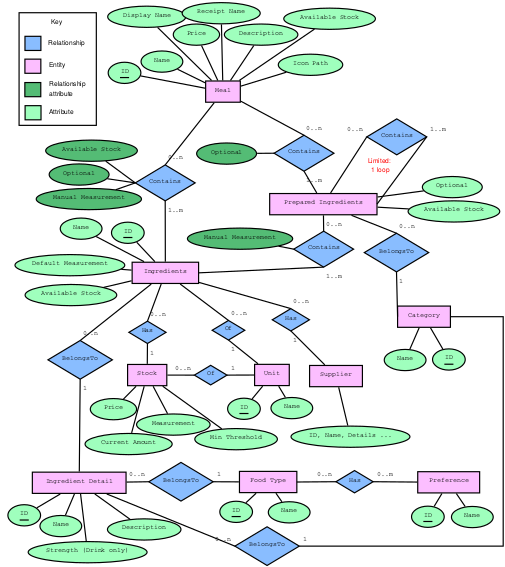
\includegraphics[height=6.5in]{/home/basedul/Documents/Report-writing-using-latex/ResturentManagementSystemReport/entityone.png}
		\caption{Entity Relationship diagram of a meal.}
		\label{fig:entityone} 
	\end{figure}
\begin{figure}[H]
		\centering
		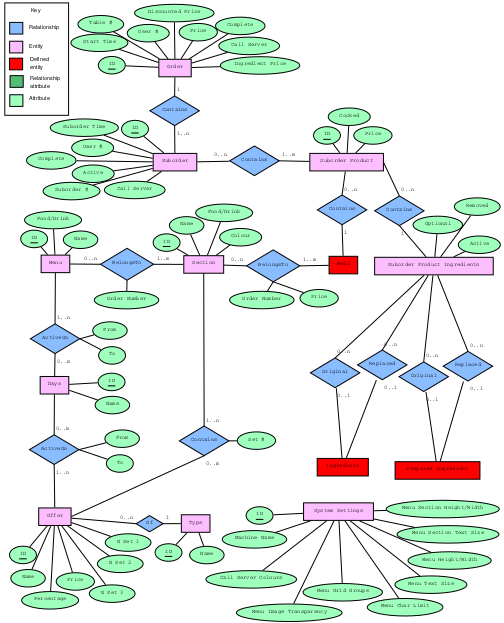
\includegraphics[height=6.5in]{/home/basedul/Documents/Report-writing-using-latex/ResturentManagementSystemReport/entitytwo.png}
		\caption{Entity Relationship of the menu, order and system settings.}
		\label{fig:entitytwo} 
	\end{figure}
	
\subsection{Graphical User Interface}	
\label{sec:guiinterface}
	The graphical user interface (GUI) is the only component of the system that the user interacts with
therefore is of great importance. The design had to be simple, clear and concise but whilst also showing
all of the required features. The main objective was to create a GUI that allowed the user to get the
order completed in the minimum time possible. This was judged by the time taken to complete the
order as well as the amount of clicks required to get from the start to the finish. In total, there are 2
different GUIs within the restaurant management system with each GUI requiring a different design
specification.
\subsubsection{Admin Gui}
The Admin system GUI has the most user interaction through the means of a touch screen. Hence
usability and user-friendliness of the GUI was of the highest priority. Therefore the specification was
as follows:\\
\begin{itemize}
	\item Chronological order of steps; either from left to right, top to bottom or a mixture of both.
	\item Minimum clicks from start to finish.
	\item Meal items.
	\item Ability to fit on any monitor size.
	\item Maximum space usage with readable font.
\end{itemize}
\begin{figure}[H]
		\centering
		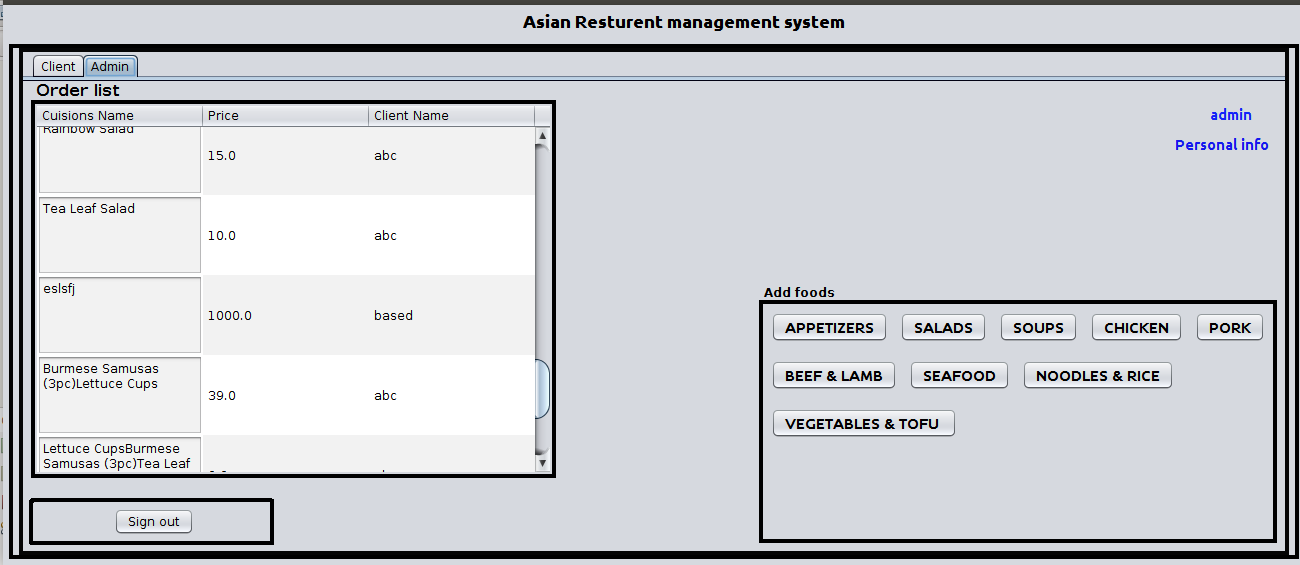
\includegraphics[height=3in]{/home/basedul/Documents/Report-writing-using-latex/ResturentManagementSystemReport/orderGui.png}
		\caption{Design of the Admin GUI for a monitor.}
		\label{fig:adminGui} 
\end{figure}
\subsubsection{Client Gui}
The Client system requires a GUI to input data therefore requires an appropriate input design.
Figure \ref{fig:clientGui} shows the design of the management application with the different functions appearing the left hand side as a tab. Each tab contains a subform with Figure 4.9 containing the structure
of the generic data input form.
\begin{figure}[H]
		\centering
		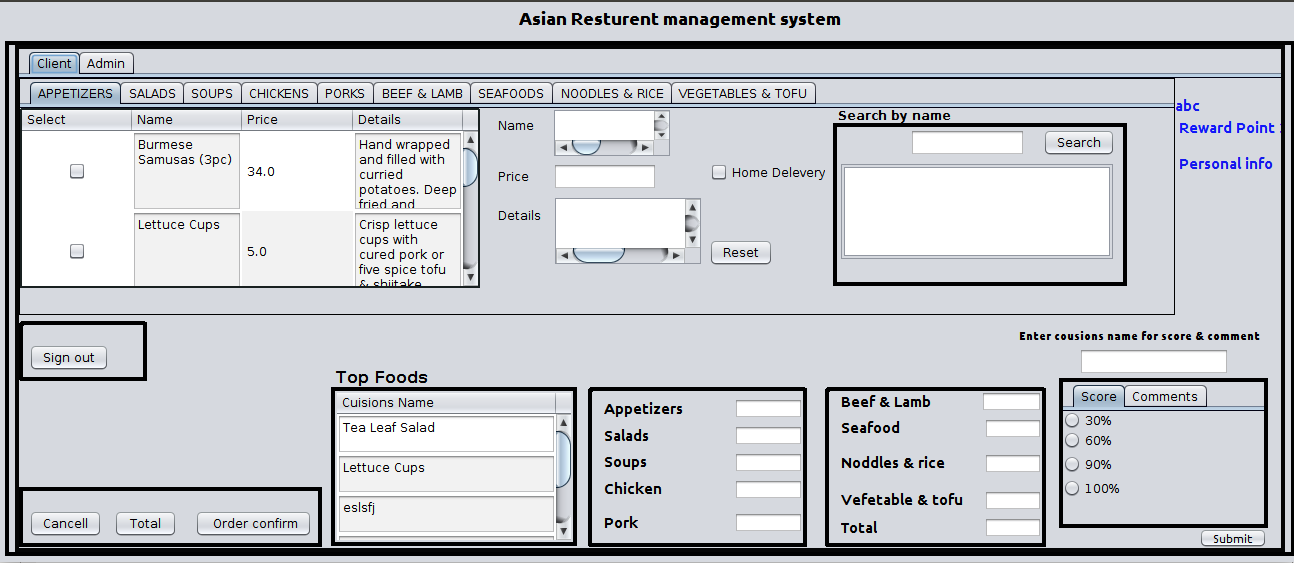
\includegraphics[height=3in]{/home/basedul/Documents/Report-writing-using-latex/ResturentManagementSystemReport/clientGui.png}
		\caption{Design of the Client GUI for a monitor.}
		\label{fig:clientGui} 
\end{figure}
	
\subsection{Flow Charts}
	A flow chart is a diagram used to represent the process flow of an algorithm, problem or some transaction
within a business. Therefore a flow chart (Figure \ref{fig:flowchart}) was used to graphically represent the process
flow of an order.
\begin{figure}[H]
		\centering
		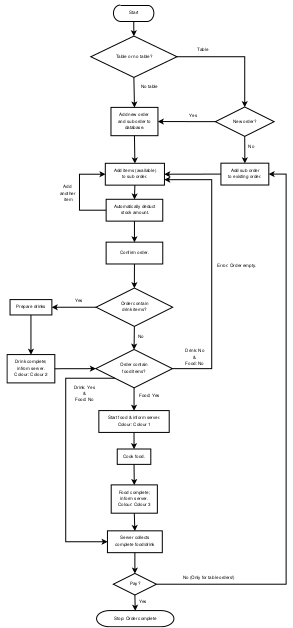
\includegraphics[height=6.5in]{/home/basedul/Documents/Report-writing-using-latex/ResturentManagementSystemReport/flowchart.png}
		\caption{Flow chart to show the flow of events of an order..}
		\label{fig:flowchart} 
\end{figure}
\end{comment}

\section{Version Control}
\tab{
	Due to the type of development methodology used for this project, incremental backups
of the system were required. Version control systems (also known as Revision control) such
as Mercurial manage the changes to documents storing each backup in its own revision
with the ability to restore back to a particular version in the event of debugging.
}

\section{Code Documentation}
\tab{
	Code documentation is an important part of any software engineering project. Throughout the implementation, a PHPDoc tool was used to generate HTML API documentation of the project.\\PHPDocumentor two\cite{Ref:17} is a tool that makes it possible to generate documentation directly from your PHP source code. With this you can provide your consumers with more information regarding the functionality embedded within your source and not just what is usable to them from your user interface.\\Documentation generated by phpDocumentor 2 does not aim to be a replacement for conventional documentation but is rather supplemental, or reference, documentation.This proves to be useful in the following example situations:

}

\section{Chapter summary}
	\tab This chapter has displayed many graphical representations of the design of the system. The implementation of the system is documented in the next chapter. 
	
	\newpage
\chapter{Tools \& Technology}
 	In the thesis project,Windows 10 used as an operating system,MySQL as a database and Visual Studio Code
as a IDE. This System is a collection of Apache server, MySQL database comprehensive programming
and easy to use.
	
	\section{Tools and technologies}
	\tab{The tools used to accomplish in this project are MySQL\cite{Ref:4}, Apache Server\cite{Ref:3} and PHP\cite{Ref:7} is Object oriented language and HTML, CSS, JavaScript}
	\subsection{MySQL database}
	\tab{MySQL\cite{Ref:4} is an open source relational database management system. It is based on the
structure query language (SQL), which is used for adding, removing, and modifying
information in the database. Standard SQL commands, such as ADD, DROP, INSERT,
and UPDATE can be used with MySQL.}\\\tab{A database is a data structure that stores organized information. Most databases
contain multiple tables, which may each include several different fields. For example, a
company database may include tables for products, employees, and financial records. Each
of these tables would have different fields that are relevant to the information stored in the
table. Today’s relational databases allow users to access, update, and search information
based on the relationship of data stored in different tables. Relational databases can also
run queries that involve multiple databases. While early databases could only store text or
such numeric data, modern databases also let users store other data types such as sound
clips, pictures, and videos.}\\\tab{SQL (Structured Query Language) is a standardized programming language used for
managing relational databases and performing various operations on the data in them.
Initially created on 1970s, SQLs is regularly being used by database administrators, as well
as by developers writing data integration scripts and data analysts looking to set up and run
analytical queries. For example, books information, client information etc}.

\subsection{Php}
	\tab{PHP\cite{Ref:5} is a server-side scripting language, especially suited for the creation of dynamic web pages. This programming language offers web developers a large selection of instruments. PHP, which has become the basis for many web applications, allows easy insertion in HTML code and connection to MySQL and PgSQL Databases.\\
	PHP was created in 1995 by Rasmus Lerdorf and means Personal Home Page language. Ever since its beginning it has been one of the most intuitive programming languages used for the creation of dynamic web pages. Later, when the PHP team was formed, the parser was rewritten and PHP version 3.0 saw the light of day. The PHP 3 version was the first serious improvement of the PHP language, which fixed a lot of bugs and completely redesigned the PHP core. The meaning of the abbreviation was also changed to PHP Hypertext Preprocessor.\\
	The launch of PHP4 marked serious progress in the usage of the programming language. This is the first version powered by the Zend Engine, which allows working with encoded files through the Zend Optimizer.\\
	The latest, so far, version 5 introduced a completely reworked, advanced object-oriented programming support, as well as many improvements towards better productivity and security. PHP 5 is an attempt to break from the PHP 3 era, while still offering almost complete backwards compatibility. Unfortunately, this PHP version still does not offer native support for Unicode or multibyte strings.\\
	NTC Hosting offers its clients an ultimate PHP hosting solution with the possibility to choose the older, but proven PHP4, or to easily upgrade to the newer PHP5. To change the PHP version, simply go to the PHP Settings menu in our Web Hosting Control Panel and select your preferred PHP revision.
}
\subsection{HTML}
		\tab{HTML\cite{Ref:7} (Hypertext Markup Language) is a text-based approach to describing how content contained within an HTML file is structured. This markup tells a web browser how to display the text, images and other forms of multimedia on a webpage.\\The role of HTML is to inform a web browser about how the content contained within an HTML file is structured. Commonly used HTML tags include <H1>, which describes a top-level heading; <H2>, which describes a second-level heading; <p> to describe a paragraph; <table>, which describes tabular data; and <ol>, which describes an ordered list of information.\\In the early days of the world wide web, marking up text-based documents using HTML syntax was more than sufficient to facilitate the sharing of academic documents and technical memos. However, as the internet expanded beyond the walls of academia and into the homes of the general population, greater demand was placed on webpages in terms of formatting and interactivity.\\HTML 4.01 was released in 1999, at a time when the internet was not yet a household name, and HTML5 was not standardized until 2014. During this time, HTML markup drifted from the job of simply describing the structure of the content on a webpage into the role of also describing how content should look when a webpage displays it.\\As a result, HTML4-based webpages often included information within a tag about what font to use when displaying text, what color should be used for the background and how content should be aligned.\\Describing within an HTML tag how an HTML element should be formatted when rendered on a webpage is considered an HTML antipattern. HTML should describe how content is structured, not how it will be styled and rendered within a browser.\\For rendering, the proper practice is to use cascading style sheets (CSS). An HTML file can link to a cascading style sheet, which will contain information about which colors to use, which fonts to use and other HTML element rendering information. Separating information about how a page is structured, which is the role of HTML, from the information about how a webpage looks when it is rendered in a browser, which is the role of a CSS file, is a software development pattern and best practice known as separation of concerns.
}		
		\subsection{CSS}
		\tab{CSS\cite{Ref:8} (Cascading Style Sheets) is used to style and layout web pages-for example, to alter the font, color, size and spacing of your content, split it into multiple columns, or add animations and other decorative features. This module gets you started on the path to CSS mastery with the basics of how it works, including selectors and properties, writing CSS rules, applying CSS to HTML, how to specify length, colour, and other units in CSS, cascade and inheritance, and debugging CSS.\\In this module we start off with a theoretical grounding, looking at what CSS is, how the browser turns HTML into a DOM, how CSS is applied to parts of the DOM, some very basic syntax examples, and what code is used to actually include our CSS in our web page.}
		\subsection{JavaScript}
		\tab{JavaScript\cite{Ref:9} works on the Client Side (on the user’s computer).\\The primary purpose of JavaScript is to provide a better experience for the user. It manipulates the objects within the HTML document. The objects and HTML elements collectively form what we call the Document Object Model (DOM). We will get into XHTML and XML later, but for now, we are going to use JavaScript with the HTML document and Cascading Styles Sheets (CSS).\\A little bit of history on JavaScript. Netscape Communications Corporation invented JavaScript back in 1995. Many different languages (from C to Python) influenced the syntax and structure of JavaScript. JavaScript is arguably one of the most flexible languages ever created. However, JavaScript is one of those languages that people claim to know, but have absolutely no idea how complex JavaScript can get. We won’t dive super far into JavaScript, but we will build a fundamental base for you.}

		\subsection{Apache server}
		\tab{Apache\cite{Ref:3} is an open-source and free web server software that powers around 46\% of websites around the world. The official name is Apache HTTP Server, and it’s maintained and developed by the Apache Software Foundation.\\It allows website owners to serve content on the web-hence the name “web server”. It’s one of the oldest and most reliable web servers, with the first version released more than 20 years ago, in 1995.\\When someone wants to visit a website, they enter a domain name into the address bar of their browser. Then, the web server delivers the requested files by acting as a virtual delivery man.\\Here at Hostinger, our web hosting infrastructure uses Apache in parallel with NGINX, which is another popular web server software. This particular setup allows us to get the best of both worlds. It greatly improves server performance by compensating the weaker sides of one software with the strengths of another.\\File servers, database servers, mail servers, and web servers use different kinds of server software. Each of these applications can access files stored on a physical server and use them for different purposes.\\The job of a web server is to serve websites on the internet. To achieve that goal, it acts as a middleman between the server and client machines. It pulls content from the server on each user request and delivers it to the web.\\The biggest challenge of a web server is to serve many different web users at the same time each of whom is requesting different pages. Web servers process files written in different programming languages such as PHP, Python, Java, and others.\\They turn them to static HTML files and serve these files in the browser of web users. When you hear the word web server, think of it as the tool responsible for the proper server-client communication.}
		
		\subsection{Visual Studio Code}
		\tab{Visual Studio Code\cite{Ref:6} combines the simplicity of a source code editor with powerful developer tooling, like Intelligence code completion and debugging.\\First and foremost, it is an editor that gets out of your way. The delightfully friction less edit-build-debug cycle means less time fiddling with your environment, and more time executing on your ideas.\\Visual Studio Code supports macOS, Linux, and Windows - so you can hit the ground running, no matter the platform.\\At its heart, Visual Studio Code features a lightning fast source code editor, perfect for day-to-day use. With support for hundreds of languages, VS Code helps you be instantly productive with syntax highlighting, bracket-matching, auto-indentation, box-selection, snippets, and more. Intuitive keyboard shortcuts, easy customization and community-contributed keyboard shortcut mappings let you navigate your code with ease.\\For serious coding, you'll often benefit from tools with more code understanding than just blocks of text. Visual Studio Code includes built-in support for Intelligence code completion, rich semantic code understanding and navigation, and code refactoring.\\And when the coding gets tough, the tough get debugging. Debugging is often the one feature that developers miss most in a leaner coding experience, so we made it happen. Visual Studio Code includes an interactive debugger, so you can step through source code, inspect variables, view call stacks, and execute commands in the console.\\VS Code also integrates with build and scripting tools to perform common tasks making everyday workflows faster. VS Code has support for Git so you can work with source control without leaving the editor including viewing pending changes diffs.\\Customize every feature to your liking and install any number of third-party extensions. While most scenarios work "out of the box" with no configuration, VS Code also grows with you, and we encourage you to optimize your experience to suit your unique needs. VS Code is an open-source project so you can also contribute to the growing and vibrant community on GitHub.\\VS Code includes enriched built-in support for Node.js development with JavaScript and TypeScript, powered by the same underlying technologies that drive Visual Studio. VS Code also includes great tooling for web technologies such as JSX/React, HTML, CSS, SCSS, Less, and JSON.\\Architecturally, Visual Studio Code combines the best of web, native, and language-specific technologies. Using Electron, VS Code combines web technologies such as JavaScript and Node.js with the speed and flexibility of native apps. VS Code uses a newer, faster version of the same industrial-strength HTML-based editor that has powered the “Monaco” cloud editor, Internet Explorer's F12 Tools, and other projects. Additionally, VS Code uses a tools service architecture that enables it to integrate with many of the same technologies that power Visual Studio, including Roslyn for .NET, TypeScript, the Visual Studio debugging engine, and more.\\Visual Studio Code includes a public extensibility model that lets developers build and use extensions, and richly customize their edit-build-debug experience.}
	\section{Chapter Summary}
	This chapter helps to understand basic idea of different tools and languages. Next Chapter gives us design concept of our House Rental Management System. 
	\newpage	
	\chapter{Conclusion}
	%\addcontentsline{toc}{section}{Conclusion}
	%{\bfseries \Large Conclusion}
	\tab {In this following chapter, we sum our work in brief and conclude the paper. We also represent a future
works which we could not able to do because of some contradictions we face during our research. We
will work more on this and we have mentioned in the future work what we tend to o next.}
	\begin{itemize}
		\item \textbf{Conclusion: }In this paper, we analyzed how the system can be made more dynamic. As the systems’ main users are
the general people so it has to be more user-friendly and dynamic. This will make life easier for the
bachelors. People do not need to roam around now for renting they can do it with some little clicks.
		\item \textbf{Future Work: }We would like make some changes in our searching. We would like to make it more dynamic. We will
add payment system and we would also like to make more use of google map for location finding.
	\end{itemize}
	
\RaggedRight \justify{On reflection, even though the majority of the proposed features were completed and
the project was deemed a huge success, the author felt that he could have been more
disciplined in keeping to the plan. He also felt that the proposed features were slightly
unrealistic and some even unnecessary. For the general project, the author felt that important aspects of research were not undertaken including interviews with house's owners
and user questionnaires. This would have provided good insight into existing solutions.\\This project has helped the author to attain new skills as well as develop existing skills.
The skills attained have been both technical and individual with the main individual skill
being project management which required good time keeping and management of the
workload.\\This chapter has concluded the project report and provided an insight into possible
future development.

}
%	\subsection{Chapter overview}
%		
%
%	\subsection{Project overview}
%	
%	\subsection{Further development}
%	
%%	\subsubsection{Graphical User Interface (GUI)}
%%	\tab Currently the GUI was adequate to do the job but maybe the GUI could have had a more appealing
%%look and feel. This all beckons on whether or not Java was the best programming language to use to
%%generate the best looking GUI. Maybe a web developed GUI could have been a better alternative but
%%with the developer having little experience in web development this would not have been ideal.
%	\subsubsection{Table management}
%	
%	\subsection{Reflection}
%	
%	\newpage
%	\subsection{Skills attained}
%	
%\subsection{Chapter summary}	

	


\newpage
\begingroup
\raggedright
\bibliography{/home/basedul/Documents/Report-writing-using-latex/HouseRentalManagementSystem/based.bib}
\bibliographystyle{IEEEtran}
\endgroup
%\newpage
%\section*{Acknowledgement}
%\addcontentsline{toc}{section}{Acknowledgement}
%	Foremost, we would like to express my sincere gratitude to the almighty Allah for His blessings and protection throughout our undergraduate studies.\\ 
%our sincere thanks to our supervisor,  \textbf{Al-Hasan} of the Institute of Computer Science and Engineering at Bangladesh Army University of Science and Technology for the continuous support of our Bachelor's study, patience, motivation, enthusiasm, and immense knowledge. His guidance helped us in all the time of research and writing of this thesis. We could not have imagined having a better advisor and mentor. We also thank our fellow classmates, our friends and for all the fun we have had in the last four years.
%        Last but not the least; We would like to thank our parents for their prayers, support, encouragement and their admonishment.\\

\end{document}
